% Options for packages loaded elsewhere
\PassOptionsToPackage{unicode}{hyperref}
\PassOptionsToPackage{hyphens}{url}
\PassOptionsToPackage{dvipsnames,svgnames,x11names}{xcolor}
%
\documentclass[
]{article}
\usepackage{amsmath,amssymb}
\usepackage{iftex}
\ifPDFTeX
  \usepackage[T1]{fontenc}
  \usepackage[utf8]{inputenc}
  \usepackage{textcomp} % provide euro and other symbols
\else % if luatex or xetex
  \usepackage{unicode-math} % this also loads fontspec
  \defaultfontfeatures{Scale=MatchLowercase}
  \defaultfontfeatures[\rmfamily]{Ligatures=TeX,Scale=1}
\fi
\usepackage{lmodern}
\ifPDFTeX\else
  % xetex/luatex font selection
\fi
% Use upquote if available, for straight quotes in verbatim environments
\IfFileExists{upquote.sty}{\usepackage{upquote}}{}
\IfFileExists{microtype.sty}{% use microtype if available
  \usepackage[]{microtype}
  \UseMicrotypeSet[protrusion]{basicmath} % disable protrusion for tt fonts
}{}
\makeatletter
\@ifundefined{KOMAClassName}{% if non-KOMA class
  \IfFileExists{parskip.sty}{%
    \usepackage{parskip}
  }{% else
    \setlength{\parindent}{0pt}
    \setlength{\parskip}{6pt plus 2pt minus 1pt}}
}{% if KOMA class
  \KOMAoptions{parskip=half}}
\makeatother
\usepackage{xcolor}
\usepackage[margin=1in]{geometry}
\usepackage{color}
\usepackage{fancyvrb}
\newcommand{\VerbBar}{|}
\newcommand{\VERB}{\Verb[commandchars=\\\{\}]}
\DefineVerbatimEnvironment{Highlighting}{Verbatim}{commandchars=\\\{\}}
% Add ',fontsize=\small' for more characters per line
\usepackage{framed}
\definecolor{shadecolor}{RGB}{248,248,248}
\newenvironment{Shaded}{\begin{snugshade}}{\end{snugshade}}
\newcommand{\AlertTok}[1]{\textcolor[rgb]{0.94,0.16,0.16}{#1}}
\newcommand{\AnnotationTok}[1]{\textcolor[rgb]{0.56,0.35,0.01}{\textbf{\textit{#1}}}}
\newcommand{\AttributeTok}[1]{\textcolor[rgb]{0.13,0.29,0.53}{#1}}
\newcommand{\BaseNTok}[1]{\textcolor[rgb]{0.00,0.00,0.81}{#1}}
\newcommand{\BuiltInTok}[1]{#1}
\newcommand{\CharTok}[1]{\textcolor[rgb]{0.31,0.60,0.02}{#1}}
\newcommand{\CommentTok}[1]{\textcolor[rgb]{0.56,0.35,0.01}{\textit{#1}}}
\newcommand{\CommentVarTok}[1]{\textcolor[rgb]{0.56,0.35,0.01}{\textbf{\textit{#1}}}}
\newcommand{\ConstantTok}[1]{\textcolor[rgb]{0.56,0.35,0.01}{#1}}
\newcommand{\ControlFlowTok}[1]{\textcolor[rgb]{0.13,0.29,0.53}{\textbf{#1}}}
\newcommand{\DataTypeTok}[1]{\textcolor[rgb]{0.13,0.29,0.53}{#1}}
\newcommand{\DecValTok}[1]{\textcolor[rgb]{0.00,0.00,0.81}{#1}}
\newcommand{\DocumentationTok}[1]{\textcolor[rgb]{0.56,0.35,0.01}{\textbf{\textit{#1}}}}
\newcommand{\ErrorTok}[1]{\textcolor[rgb]{0.64,0.00,0.00}{\textbf{#1}}}
\newcommand{\ExtensionTok}[1]{#1}
\newcommand{\FloatTok}[1]{\textcolor[rgb]{0.00,0.00,0.81}{#1}}
\newcommand{\FunctionTok}[1]{\textcolor[rgb]{0.13,0.29,0.53}{\textbf{#1}}}
\newcommand{\ImportTok}[1]{#1}
\newcommand{\InformationTok}[1]{\textcolor[rgb]{0.56,0.35,0.01}{\textbf{\textit{#1}}}}
\newcommand{\KeywordTok}[1]{\textcolor[rgb]{0.13,0.29,0.53}{\textbf{#1}}}
\newcommand{\NormalTok}[1]{#1}
\newcommand{\OperatorTok}[1]{\textcolor[rgb]{0.81,0.36,0.00}{\textbf{#1}}}
\newcommand{\OtherTok}[1]{\textcolor[rgb]{0.56,0.35,0.01}{#1}}
\newcommand{\PreprocessorTok}[1]{\textcolor[rgb]{0.56,0.35,0.01}{\textit{#1}}}
\newcommand{\RegionMarkerTok}[1]{#1}
\newcommand{\SpecialCharTok}[1]{\textcolor[rgb]{0.81,0.36,0.00}{\textbf{#1}}}
\newcommand{\SpecialStringTok}[1]{\textcolor[rgb]{0.31,0.60,0.02}{#1}}
\newcommand{\StringTok}[1]{\textcolor[rgb]{0.31,0.60,0.02}{#1}}
\newcommand{\VariableTok}[1]{\textcolor[rgb]{0.00,0.00,0.00}{#1}}
\newcommand{\VerbatimStringTok}[1]{\textcolor[rgb]{0.31,0.60,0.02}{#1}}
\newcommand{\WarningTok}[1]{\textcolor[rgb]{0.56,0.35,0.01}{\textbf{\textit{#1}}}}
\usepackage{longtable,booktabs,array}
\usepackage{calc} % for calculating minipage widths
% Correct order of tables after \paragraph or \subparagraph
\usepackage{etoolbox}
\makeatletter
\patchcmd\longtable{\par}{\if@noskipsec\mbox{}\fi\par}{}{}
\makeatother
% Allow footnotes in longtable head/foot
\IfFileExists{footnotehyper.sty}{\usepackage{footnotehyper}}{\usepackage{footnote}}
\makesavenoteenv{longtable}
\usepackage{graphicx}
\makeatletter
\def\maxwidth{\ifdim\Gin@nat@width>\linewidth\linewidth\else\Gin@nat@width\fi}
\def\maxheight{\ifdim\Gin@nat@height>\textheight\textheight\else\Gin@nat@height\fi}
\makeatother
% Scale images if necessary, so that they will not overflow the page
% margins by default, and it is still possible to overwrite the defaults
% using explicit options in \includegraphics[width, height, ...]{}
\setkeys{Gin}{width=\maxwidth,height=\maxheight,keepaspectratio}
% Set default figure placement to htbp
\makeatletter
\def\fps@figure{htbp}
\makeatother
\setlength{\emergencystretch}{3em} % prevent overfull lines
\providecommand{\tightlist}{%
  \setlength{\itemsep}{0pt}\setlength{\parskip}{0pt}}
\setcounter{secnumdepth}{5}
\newlength{\cslhangindent}
\setlength{\cslhangindent}{1.5em}
\newlength{\csllabelwidth}
\setlength{\csllabelwidth}{3em}
\newlength{\cslentryspacingunit} % times entry-spacing
\setlength{\cslentryspacingunit}{\parskip}
\newenvironment{CSLReferences}[2] % #1 hanging-ident, #2 entry spacing
 {% don't indent paragraphs
  \setlength{\parindent}{0pt}
  % turn on hanging indent if param 1 is 1
  \ifodd #1
  \let\oldpar\par
  \def\par{\hangindent=\cslhangindent\oldpar}
  \fi
  % set entry spacing
  \setlength{\parskip}{#2\cslentryspacingunit}
 }%
 {}
\usepackage{calc}
\newcommand{\CSLBlock}[1]{#1\hfill\break}
\newcommand{\CSLLeftMargin}[1]{\parbox[t]{\csllabelwidth}{#1}}
\newcommand{\CSLRightInline}[1]{\parbox[t]{\linewidth - \csllabelwidth}{#1}\break}
\newcommand{\CSLIndent}[1]{\hspace{\cslhangindent}#1}
\usepackage{caption}
\usepackage{booktabs}
\usepackage{longtable}
\usepackage{array}
\usepackage{multirow}
\usepackage{wrapfig}
\usepackage{float}
\usepackage{colortbl}
\usepackage{pdflscape}
\usepackage{tabu}
\usepackage{threeparttable}
\usepackage{threeparttablex}
\usepackage[normalem]{ulem}
\usepackage{makecell}
\usepackage{xcolor}
\ifLuaTeX
  \usepackage{selnolig}  % disable illegal ligatures
\fi
\IfFileExists{bookmark.sty}{\usepackage{bookmark}}{\usepackage{hyperref}}
\IfFileExists{xurl.sty}{\usepackage{xurl}}{} % add URL line breaks if available
\urlstyle{same}
\hypersetup{
  pdftitle={Sleep, relative to wake, increases both veridical and false memory in the DRM paradigm: A registered report},
  pdfauthor={Matthew H.C. Mak, Alice O'Hagan, Aidan J. Horner, M. Gareth Gaskell},
  colorlinks=true,
  linkcolor={black},
  filecolor={Maroon},
  citecolor={Blue},
  urlcolor={Blue},
  pdfcreator={LaTeX via pandoc}}

\title{Sleep, relative to wake, increases both veridical and false memory in the DRM paradigm: A registered report}
\author{Matthew H.C. Mak, Alice O'Hagan, Aidan J. Horner, M. Gareth Gaskell}
\date{Department of Psychology, University of York, UK}

\begin{document}
\maketitle

\hypertarget{author-note}{%
\section*{Author Note}\label{author-note}}
\addcontentsline{toc}{section}{Author Note}

We have no conflict of interest to disclose. Correspondence concerning this article should be addressed to Matthew Mak, Department of Psychology, University of York, Heslington, York, YO10 5DD, United Kingdom; Email: \url{matthew.mak@york.ac.uk}

\hypertarget{acknowledgements}{%
\section*{Acknowledgements}\label{acknowledgements}}
\addcontentsline{toc}{section}{Acknowledgements}

This research was supported by a BA/Leverhulme Small Research Grant (Number: SRG21\textbackslash210150) awarded to Matthew Mak and Gareth Gaskell, who were also supported by a grant from the Economic and Social Research Council (ESRC; ES/T008571/1). Aidan Horner was supported by an ESRC grant (ES/R007454/1). The funders have no role in study design, data collection and analysis, decision to publish or preparation of the manuscript. We would like to express our gratitude to members of the SLAM group for their valuable discussions regarding this work, as well as extend our thanks to the four reviewers for providing constructive feedback on this study.

\hypertarget{open-science-statement}{%
\section*{Open Science Statement}\label{open-science-statement}}
\addcontentsline{toc}{section}{Open Science Statement}

All the materials, data, and analysis scripts are publicly available on Open Science Framework (\url{https://osf.io/9pdyf/}).

\hypertarget{abstract}{%
\section*{Abstract}\label{abstract}}
\addcontentsline{toc}{section}{Abstract}

Human memory is known to be supported by sleep. However, less is known about the effect of sleep on false memory, where people remember events that never occurred. In the laboratory, false memories are often induced via the Deese-Roediger-McDermott (DRM) paradigm where participants are presented with semantically related words such as nurse, hospital, and sick (studied words). Subsequently, participants are likely to falsely remember that a related lure word such as doctor was presented. Multiple studies have examined whether these false memories are influenced by sleep, with contradictory results. A recent meta-analysis suggests that sleep may increase DRM false memory when short lists are used. We tested this in a registered report (N=488) with a 2 (Interval: Immediate vs.~12-hr Delay) \(\times\) 2 (Test Time: 9AM vs.~9PM) between-participant DRM experiment, using short DRM lists (N = 8 words/list) and free recall as the memory test. We found that the Sleep and Wake participants were well-matched on the number of total responses, but those in the Sleep group produced fewer intrusions (i.e., words that were neither studied nor lure words), and when this was statistically controlled for, they showed a greater tendency to recall more critical lures as well as more studied items. Our findings support the view that sleep may facilitate gist abstraction and/or spreading activation, alongside strengthening/protecting newly encoded declarative memories.

\textbf{Keywords}: Sleep, False Memory, DRM, Recall, Gist Abstraction, Spreading Activation

\hypertarget{experiment}{%
\section*{Experiment}\label{experiment}}
\addcontentsline{toc}{section}{Experiment}

\hypertarget{overview}{%
\section{Overview}\label{overview}}

It is possible to index DRM false memory via free recall or recognition (e.g., Stadler et al., 1999). In this experiment, we used free recall only, because recall tends to be more prone to sleep-related memory effects than recognition {[}\protect\hyperlink{ref-newbury2019a}{1}--\protect\hyperlink{ref-lipinska2019a}{3},\protect\hyperlink{ref-berres2021a}{\textbf{berres2021a?}}{]}. Our experiment comprised a study and a test phase. In the study phase, a participant encoded 20 short DRM wordlists, with each containing 8 words. Short lists were chosen because Newbury and Monaghan's {[}\protect\hyperlink{ref-newbury2019a}{1}{]} meta-analysis pinpointed a clear sleep effect in these lists. In the test phase, participants recalled the wordlists in a free recall procedure.

Participants were randomly assigned to one of the four groups: AM-control, PM-control, Sleep, or Wake. Those assigned to the control (aka Immediate) groups carried out the test phase immediately after the study phase, with those in the AM group starting at 9AM (± 1hr) and those in the PM group starting at 9PM (± 1hr). No difference in false or veridical recall was expected between these groups, as prior DRM studies (e.g., {[}\protect\hyperlink{ref-fenn2009a}{4}--\protect\hyperlink{ref-payne2009a}{6}{]}) have consistently demonstrated that immediate recall was equivalent between morning and evening. The inclusion of these control groups helped rule out potential circadian effects on encoding and retrieval (and relatedly, monitoring in the Activation/Monitoring Framework). Finally, participants assigned to the Sleep and Wake groups (collectively referred to as the Delay groups) started the test phase approximately 12 hours after the study phase. Those in the Wake group studied the DRM wordlists in the morning (9AM ± 1hr) and completed the test phase in the evening (9PM ± 1hr) on the same day. Those in the Sleep group encoded the wordlists in the evening (9PM ± 1hr) and completed the test phase in the morning (9AM ± 1hr) the next day.

\hypertarget{research-questions-and-corresponding-predictions}{%
\section{Research questions and corresponding predictions}\label{research-questions-and-corresponding-predictions}}

This experiment set out to address a key question:

\(\text{\underline{\#1 Does overnight sleep (vs. daytime wakefulness) influence DRM false recall?}}\)

Our prediction was based on the meta-analysis by Newbury and Monaghan {[}\protect\hyperlink{ref-newbury2019a}{1}{]}, who reported that when a study used short lists, sleep consistently increased DRM false memory. We, therefore, predicted a post-sleep (vs.~post-wake) increase in DRM false recall, whereas there would be no such difference between the AM- and PM-control groups.

Our study also addressed a peripheral question:

\(\text{\underline{\#2 Does overnight sleep (vs. daytime wakefulness) increase veridical recall of the studied list words?}}\)

Again, our prediction is based on Newbury and Monaghan {[}\protect\hyperlink{ref-newbury2019a}{1}{]}, who found that sleep benefits veridical memory in short lists. Our prediction to this question was, therefore that veridical recall would be greater post-sleep than post-wake, whereas there would be no such difference between the AM- and PM-control groups.

\hypertarget{design}{%
\section{Design}\label{design}}

\(\text{\underline{\#1 Does overnight sleep (vs. daytime wakefulness) influence DRM false recall?}}\)

For this question, the dependent variable was whether a critical lure is recalled or not (i.e., binary). There were two independent variables: Interval (Immediate vs.~Delay) and Test Time (9AM vs.~9PM), both of which were manipulated between-participants. In other words, the four groups were coded as in Table \ref{tab:table1}:

\begin{table}[H]

\caption{\label{tab:table1}How the four groups were coded using Interval and Test Time.}
\centering
\begin{tabular}[t]{ccccc}
\toprule
\textbf{Groups} & \textbf{ } & \textbf{Interval} & \textbf{ } & \textbf{Test Time}\\
\midrule
AM-control & = & Immediate & + & 9AM\\
PM-control & = & Immediate & + & 9PM\\
Sleep & = & Delay & + & 9AM\\
Wake & = & Delay & + & 9PM\\
\bottomrule
\end{tabular}
\end{table}

To address Research Question \#1, we first tested if any difference between the Sleep and Wake groups was significantly different from that between the AM- and PM-control groups (i.e., an interaction between Interval and Test Time). This is important because it allows us to rule out time-of-day effects. Then, we tested for the simple effect of Test Time (9AM vs.~9PM) within the Immediate and Delay groups. If there is (1) a significant Interval x Test Time interaction and (2) a significant Test Time effect within the Delay groups (Sleep \textgreater{} Wake), we will be able conclude that sleep (but not time-of-day) increases false recall.\footnote{Prior studies in the ‘Sleep $\times$ DRM’ literature (e.g., Fenn et al., 2009; Payne et al., 2009) conducted two separate statistical tests, one comparing Sleep vs. Wake, another comparing AM- vs. PM- controls. They then concluded that Sleep had an effect on DRM false memory beyond time-of-day effects when Test Time was significant in the Sleep vs. Wake comparison ($p$ < 0.05) but not in the AM vs. PM comparison ($p$ > 0.05). Unfortunately, however, this is not sufficient (Nieuwenhuis et al., 2011), as “the difference between ‘significant’ and ‘not significant’ is not itself statistically significant” (Gelmam \& Stern, 2006). Therefore, in order to rule out time-of-day effects, one needs to show that Sleep vs. Wake is significantly different from AM vs. PM-control. This can be captured by an Interval $\times$ Test Time interaction.}

\(\text{\underline{\#2 Does overnight sleep (vs. daytime wakefulness) increase veridical recall of the studied list words?}}\)

For this research question, the dependent variable was whether a studied list word was recalled or not (i.e., binary). As per Question \#1, there were two between-participant manipulations: Interval (Immediate vs.~Delay) and Test Time (9AM vs.~9PM). We first tested if there was an interaction between Interval and Test Time. Then, we tested for the simple effect of Test Time within the Immediate and Delay groups. Note that this research question is secondary to the first.

\hypertarget{target-sample-size-and-stopping-rules}{%
\section{Target sample size and stopping rules}\label{target-sample-size-and-stopping-rules}}

Our target sample size was 120 participants/group (i.e., 480 participants in total), defined as those who remained in the sample after applying the exclusion criteria outlined in section 9. This sample size gives us \textgreater=90\% power to detect all the desired effects for our Research Questions (See Appendix D for a detailed power analysis).

\hypertarget{recruitment}{%
\section{Recruitment}\label{recruitment}}

\hypertarget{online-recruitment.}{%
\subsection{Online recruitment.}\label{online-recruitment.}}

Participants were recruited online via Prolific (\url{https://www.prolific.co/}). All participants completed the experiment unsupervised and at a location of their own choosing. We chose online testing, as opposed to lab-based testing, for at least two reasons. First, given the unpredictability of the COVID-19 pandemic, we did not want to risk the possibility of data collection being disrupted. Second, given the time limit on the funding for this work, it would have been logistically difficult to reach the target sample size were the study conducted in person.

One key concern associated with online testing is data quality. This stems from the fact that researchers cannot monitor participants during an online experiment. However, it has been repeatedly demonstrated that as long as appropriate measures are taken (e.g., {[}\protect\hyperlink{ref-rodd2019a}{7},\protect\hyperlink{ref-curtis2022a}{8}{]}), data quality from online experiments is no different from lab-based experiments (e.g., {[}\protect\hyperlink{ref-anwyl-irvine2020a}{9}--\protect\hyperlink{ref-mak2021b}{12}{]}). Furthermore, two recent online studies using the same experimental design {[}\protect\hyperlink{ref-ashton2021a}{13},\protect\hyperlink{ref-mak2023a}{\textbf{mak2023a?}}{]} found clear evidence of a sleep benefit in the classic paired-associate learning paradigm, replicating well-established evidence from lab-based experiments (e.g., {[}\protect\hyperlink{ref-lo2014a}{14},\protect\hyperlink{ref-plihal1997a}{15}{]}). Importantly, the effect sizes for sleep from these online studies were roughly equivalent to those reported by lab-based studies. Together, these suggest that it is possible to detect sleep-related memory effects in online experiments, as long as the appropriate measures are put in place. These are detailed in the Procedures section (\#8) below.

\hypertarget{recruitment-method.}{%
\subsection{Recruitment method.}\label{recruitment-method.}}

Following two previous sleep studies conducted via Prolific {[}\protect\hyperlink{ref-mak2023a}{\textbf{mak2023a?}},\protect\hyperlink{ref-mak2023b}{\textbf{mak2023b?}}{]}, we put a short survey on the platform to recruit a pool of participants (N = 2296). This survey is available in Appendix A and was hosted on Qualtrics. The first half of the survey asked for basic demographic information: gender identity, age, current country of residence, first language, ethnicity, highest education attainment, and history of developmental/sleep disorders (if any). The survey then provided a brief outline of the main study. It stated that if enrolled, participants would be randomly allocated to one of the four groups and that no preferences would be accommodated. Participants then indicated whether they would like to enrol in the main study. Of the 2296 respondents, 1940 expressed interest in taking part, who were then screened for their eligibility (see inclusion criteria below). Those who fitted our inclusion criteria were then randomly allocated to one of the four experimental groups. A private message was sent to each participant, notifying them of their group allocation. In the end, 534 participants completed both the study and test phases. These participants were reimbursed at a rate of \textasciitilde£9.5/hr.

\hypertarget{inclusion-criteria}{%
\section{Inclusion criteria}\label{inclusion-criteria}}

We applied these inclusion criteria to ensure comparability with prior studies (e.g., {[}\protect\hyperlink{ref-fenn2009a}{4},\protect\hyperlink{ref-payne2009a}{6},\protect\hyperlink{ref-mckeon2012a}{16},\protect\hyperlink{ref-shaw2017a}{17}{]}):

\begin{enumerate}
\def\labelenumi{\arabic{enumi}.}
\item
  Aged 18-25
\item
  Speaks English as (one of) their first language(s)
\item
  No known history of any psychiatric (e.g., schizophrenia), developmental (e.g., dyslexia) or sleep (e.g., insomnia) disorders
\item
  Currently resides in the UK, indexed by their IP address (since this experiment requires participants to complete each phase at a certain time of day, it is necessary to restrict the location to prevent participants from taking the study in different time zones)
\item
  Normal vision or corrected-to-normal vision
\item
  Normal hearing
\item
  Able to complete the study using a laptop or a desktop PC
\item
  Able to complete both the study and test phases
\item
  Has an approval rate of \textgreater96\% on Prolific. This helps ensure that a participant has a tendency to take online studies seriously.
\end{enumerate}

\hypertarget{materials}{%
\section{Materials}\label{materials}}

Prior studies in the DRM literature typically showed 8 to 15 words per list (e.g., {[}\protect\hyperlink{ref-fenn2009a}{4},\protect\hyperlink{ref-shaw2017a}{17},\protect\hyperlink{ref-swannell2013a}{18}{]}). Generally, within this range, showing fewer words reduces false recall rates ({[}\protect\hyperlink{ref-swannell2013a}{18},\protect\hyperlink{ref-robinson1997a}{19}{]}; see also {[}\protect\hyperlink{ref-alakbarova2021a}{20}{]}). However, showing even fewer words per list (e.g., 3) results in floor or near-floor rates {[}\protect\hyperlink{ref-robinson1997a}{19}{]}. Given that sleep seems to have a larger effect on false memory when the gist trace or lure is encoded at a medium level during study {[}\protect\hyperlink{ref-newbury2019a}{1}{]}, we opted for 8 words per list.

We made use of 20 DRM wordlists (see Table \ref{tab:table2}), taken from Roediger et al. {[}\protect\hyperlink{ref-roediger2001a}{21}{]}. Each list contained 8 semantically related words, and as per the standard DRM paradigm, they were arranged in a descending order of associative strength to the critical lures. A participant studied all 20 lists. We note that the original DRM lists by Roediger et al. {[}\protect\hyperlink{ref-roediger2001a}{21}{]} were tailored for American participants, and two words (e.g., trash, Mississippi) were not immediately relatable to people in the UK. We, therefore, changed these words (e.g., trash → rubbish), as noted in Table \ref{tab:table2}.

We acknowledge that previous studies in the `Sleep \(\times\) DRM' literature typically showed participants 8 to 16 lists (e.g., {[}\protect\hyperlink{ref-payne2009a}{6},\protect\hyperlink{ref-mckeon2012a}{16}{]}), so our participants studied more wordlists (i.e., 20). However, since we showed relatively few words per list, the total number of studied words was comparable to prior studies (i.e., 160 in the current vs.~96 to 225 in prior studies). Furthermore, an advantage of showing more wordlists is that more critical lures could be recalled (i.e., 20 lists = 20 lures), potentially increasing variability between participants and hence our ability to detect sleep-related effects.

\hypertarget{procedures}{%
\section{Procedures}\label{procedures}}

The procedure of the study is summarised in Figure \ref{fig:expprocedure}. The study was hosted on Gorilla (www.gorilla.sc; {[}\protect\hyperlink{ref-anwyl-irvine2020a}{9}{]}). A study phase took approximately 11 minutes. Here, participants first gave informed consent, completed a language/attention check, rated their level of sleepiness on the Stanford Sleepiness Scale (SSS; {[}\protect\hyperlink{ref-hoddes1973a}{22}{]}), and viewed 20 DRM wordlists.

Immediately afterwards, participants in the AM/PM-control groups carried out the test phase. For those in the Delay groups, the test phase took place approximately 12 hours later. Here, both the Immediate and Delay participants rated their level of sleepiness on SSS and completed a short survey concerned with, for example, morningness/eveningness preference (rMEQ; {[}\protect\hyperlink{ref-adan1991a}{23}{]}) and sleep duration/quality the night before (see Appendix B for the full survey). This survey helped determine whether the four groups were matched in terms of time-of-day preference and whether data from a participant needed to be discarded as a result of meeting the exclusion criteria described in section 9. Finally, the test phase concluded with a 10-minute free recall task where participants recalled as many of the words as they could from the previously seen wordlists.

\begin{figure}

{\centering 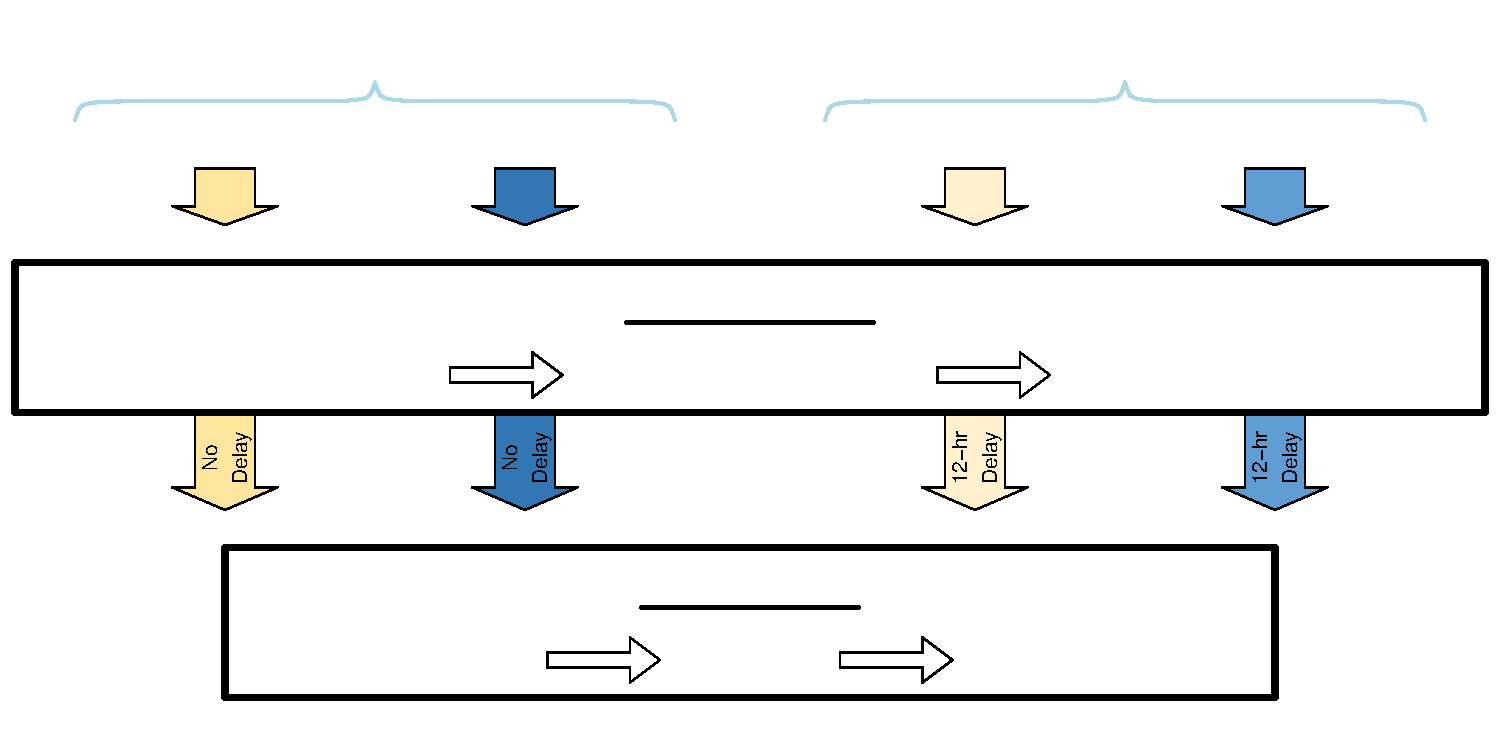
\includegraphics{Figures/expprocedure} 

}

\caption{Experimental procedure.}\label{fig:expprocedure}
\end{figure}

\hypertarget{exposure-to-the-drm-wordlists.}{%
\subsection{Exposure to the DRM wordlists.}\label{exposure-to-the-drm-wordlists.}}

On the instruction page, participants were told that they would see some English words presented one after the other on the computer screen. They were asked to pay close attention to the words because they would be tested on them later on. No specific instruction was given regarding the subsequent test format.

During presentation, words in each DRM list were presented visually,\footnote{Newbury and Monaghan [@newbury2019a] found no evidence in their meta-analysis that the modality of presentation modulated the effect of sleep. However, in a set of three experiments, Fenn et al. [@fenn2009a] used auditory presentation in one of them and visual in the other two. As far as we are aware, this is the only study in the ‘Sleep $\times$ DRM’ literature that had used both modalities in the same set of experiments. Sleep appeared to have a larger effect on false memory when visual (vs. auditory) presentation was used. Given this, we opted for visual presentation in the current experiment.} in a fixed order and arranged in descending associative strength to the unpresented critical lure (see Table \ref{tab:table2} for order). Each list began with a fixation for 1 s, followed by the first word in a list. Each word was shown for 1 s, in a lowercase black font (Arial, size 26) on a white background, and separated by a 500-ms interstimulus interval. After presentation of the final word in a list was 5 s of blank screen. List order was randomised, and each list was seen once.

\begin{table}[H]

\caption{\label{tab:table2}The 20 DRM wordlists to be used.}
\centering
\begin{tabular}[t]{lll}
\toprule
\textbf{Critical lure} & \textbf{False recall probability} & \textbf{List items (arranged in the}\\
\textbf{of each list} & \textbf{(Roediger et al. 2001)} & \textbf{order of presentation in study)}\\
\midrule
\em{Window} & \em{65} & \em{door, glass, pane, shade, ledge, sill, house, open}\\
\em{Sleep} & \em{61} & \em{bed, rest, awake, tired, dream, wake, snooze, blanket}\\
\em{Doctor} & \em{60} & \em{nurse, sick, lawyer, medicine, health, hospital, dentist, physician}\\
\addlinespace
\em{Smell} & \em{60} & \em{nose, breathe, sniff, aroma, hear, see, nostril, whiff}\\
\em{Chair} & \em{54} & \em{table, sit, legs, seat, couch, desk, recliner, sofa}\\
\em{Smoke} & \em{54} & \em{cigarette, puff, blaze, billows, pollution, ashes, cigar, chimney}\\
\em{Sweet} & \em{54} & \em{sour, candy, sugar, bitter, good, taste, tooth, nice}\\
\em{Rough} & \em{53} & \em{smooth, bumpy, road, tough, sandpaper, jagged, ready, coarse}\\
\addlinespace
\em{Needle} & \em{52} & \em{thread, pin, eye, sewing, sharp, point, prick, thimble}\\
\em{Rubbish} & \em{49} & \em{garbage, waste, can, refuse, sewage, bag, junk, trash (Note 1)}\\
\em{Anger} & \em{49} & \em{mad, fear, hate, rage, temper, fury, ire, wrath}\\
\em{Soft} & \em{46} & \em{hard, light, pillow, plush, loud, cotton, fur, touch}\\
\em{City} & \em{46} & \em{town, crowded, state, capital, streets, subway, country, New York}\\
\addlinespace
\em{Cup} & \em{45} & \em{mug, saucer, tea, measuring, coaster, lid, handle, coffee}\\
\em{Cold} & \em{44} & \em{hot, snow, warm, winter, ice, wet, frigid, chilly}\\
\em{Mountain} & \em{42} & \em{hill, valley, climb, summit, top, molehill, peak, plain}\\
\em{Slow} & \em{42} & \em{fast, lethargic, stop, listless, snail, cautious, delay, traffic}\\
\em{River} & \em{42} & \em{water, stream, lake, Thames (Note 2), boat, tide, swim, flow}\\
\addlinespace
\em{Spider} & \em{37} & \em{web, insect, bug, fright, fly, arachnid, crawl, tarantula}\\
\em{Foot} & \em{35} & \em{shoe, hand, toe, kick, sandals, soccer, yard, walk}\\
\bottomrule
\multicolumn{3}{l}{\textsuperscript{} Note 1. In Roediger et al. (2001), the critical lure for this list was trash, with rubbish being one of the list}\\
\multicolumn{3}{l}{items. We used rubbish as the critical lure and trash as a list item because the former is the preferred term in}\\
\multicolumn{3}{l}{British English.}\\
\multicolumn{3}{l}{\textsuperscript{} Note 2. The original word in Roediger et al. was Mississippi. We replaced it with Thames.}\\
\end{tabular}
\end{table}

There was a surprise attention check after the 4th, 9th, 13th, 18th lists, where participants saw an erroneous maths equation such as ``3 + 3 = 11''. It was presented for 1 s, in the same font and style as the list words {[}\protect\hyperlink{ref-thomas2017a}{24}{]}. Immediately afterwards, participants were asked to report what 3 + 3 was according to what was just shown.

\hypertarget{free-recall.}{%
\subsection{Free Recall.}\label{free-recall.}}

Participants had 10 mins to type out all the words they could remember from the study phase in a textbox. When there was 2 min left, a timer appeared. Participants could not proceed before the time was up.
To maximise the likelihood that participants paid full attention instead of doing something else (e.g., playing with their phone) during recall, there was an attention check throughout: On the same page as the response textbox, there was a white square that turned red every 2 to 3 mins. The change in colour lasted for 10 s, during which a single digit was shown. Participants had to enter the digit into a separate textbox to show that they were paying attention. Throughout the 10-min recall task, the square turned red four times, so participants needed to enter four digits as they attempted the recall task.

\hypertarget{additional-measures-to-ensure-data-quality.}{%
\subsection{Additional measures to ensure data quality.}\label{additional-measures-to-ensure-data-quality.}}

At the start of the study phase, participants were encouraged to take the experiment seriously and were informed that their participation would contribute to science. After rating their level of sleepiness, participants must pass a language/attention check. This involved the auditory presentation of a short story. Replay and pausing were not permitted. Participants then answered two simple comprehension questions based on the story. Failure to answer both questions correctly led to their data being excluded from further analysis. These questions helped to ensure that participants could indeed understand English and were in a reasonably quiet environment. Next, to prevent participants from multitasking on the computer, both the study and test phases required participants to enter full-screen mode. Participants were told that exit from full-screen mode during the study may lead to no payment. This was made possible by Gorilla, which recorded the browser's and the monitor's sizes. At the end of the study phase, participants were asked to describe how they learnt the words in a sentence. Participants who said they wrote down or similarly recorded the words were excluded from further analysis.

\hypertarget{exclusion-criteria}{%
\section{Exclusion criteria}\label{exclusion-criteria}}

Exclusion was applied on the participant level. A participant's dataset was excluded from further analysis and replaced, if

\begin{enumerate}
\def\labelenumi{\arabic{enumi}.}
\item
  they exited full-screen mode in any of the phases.
\item
  they failed the language/attention check at the start of the study.
\item
  they reported to have written down or recorded the wordlists during the study phase.
\item
  (Sleep and Wake groups only) they reported consuming any alcoholic drinks between study and test.
\item
  (Sleep group only) they reported to have had fewer than 6 hours of overnight sleep prior to test or rated their sleep quality as poor or extremely poor.
\item
  (Wake group only) they reported to have had a nap between study and test.
\item
  they failed more than one of the four attention checks (i.e., 3 + 3 = 11) at study.
\item
  they failed to report more than one of the four digits in the attention check of free recall.
\item
  they submitted a blank response in free recall.
\item
  (this criterion was removed; see Deviations from Stage-1 registered report on p.~1 for explanation)
\item
  their completion time for either the study or test phase is 3 standard deviations above or below their respective mean completion time of the first 480 participants who completed the study.
\end{enumerate}

\hypertarget{participants}{%
\section{Participants}\label{participants}}

Of the 534 participants who completed both the study and test phases, 46 were excluded for meeting one or more of the exclusion criteria. The full list of excluded participants and their respective reason for exclusion is available on OSF (see exclusion\_OSF.csv). Our final sample size comprised 488 participants, with 124 in each of the Immediate groups, and 120 in each of the Delay groups. Group characteristics are summarised in Table \ref{tab:table3}.

\begin{table}[H]

\caption{\label{tab:table3}Group characteristics.}
\centering
\fontsize{9}{11}\selectfont
\begin{tabular}[t]{lcccc}
\toprule
Characteristics & Immediate & Immediate & Sleep (aka & Wake (aka\\
 & -AM & -PM & Delay-AM) & Delay-PM)\\
\midrule
N before exclusion & 130 & 127 & 135 & 143\\
N after exclusion & 124 & 124 & 120 & 120\\
Mean age (SD) & 22.24 (2.18) & 22.34 (2.03) & 22.18 (1.93) & 22.25 (1.93)\\
\addlinespace
Gender (Female:Male:Other) & 64 : 54 : 2 & 77 : 46 : 1 & 62 : 57 : 1 & 58 : 61 : 1\\
\% participants identified as ethnically white & 78.2\% & 73.4\% & 81.7\% & 80\%\\
Mean SSS rating at study (SD) & 2.58 (0.98) & 2.64 (1.12) & 2.66 (0.96) & 2.58 (0.98)\\
Mean SSS rating at test (SD) & 2.73 (1.04) & 2.95 (1.29) & 2.63 (1.21) & 2.67 (1.18)\\
Mean rMEQ score (SD) & 15.89 (1.67) & 15.59 (1.91) & 15.72 (1.83) & 15.53 (1.99)\\
\addlinespace
Mean N of intervening hr between study and test (SD) & NA & NA & 12.22 (0.74) & 12.14 (0.81)\\
\bottomrule
\multicolumn{5}{l}{\textsuperscript{} Notes. (1) SSS stands for Stanford Sleepiness Scale and ranges from 1 to 6, with higher values indicating}\\
\multicolumn{5}{l}{greater sleepiness. (2) rMEQ stands for reduced Morningness/Eveningness Questionnaire; it ranges from 1}\\
\multicolumn{5}{l}{to 25, with higher values indicating greater morningness preference.}\\
\end{tabular}
\end{table}

Prior to the confirmatory analyses, we first checked if the four groups were matched on their morningness/eveningness preference and degree of sleepiness at study/test (as indexed by the Stanford Sleepiness Scale). These are summarised in Table \ref{tab:table3}. We compared the four groups on each of the measures using one-way ANOVAs, which showed no significant differences (SSS at study: F = 0.21, p = .888; SSS at test: F = 1.63, p = .183; rMEQ: F = 0.97, p = .408). We also compared the Sleep and Wake groups on the number of intervening hours between study and test using a between-participant t-test, which revealed no significant difference {[}t(236.16) = 0.86, p = .389{]}. In sum, our four groups were well-matched on these potentially confounding factors.

\hypertarget{data-pre-processing}{%
\section{Data pre-processing}\label{data-pre-processing}}

The free recall data were pre-processed. The first step was to remove any duplicate responses. The second was to correct all obvious spelling and typing errors to the nearest English words, defined as Levenstein distance \(\leq\) 2 (e.g., *cigerette → cigarette).\footnote{If a misspelt response has more than one nearest word, the response was considered as an intrusion.} Responses with added or dropped inflectional suffixes (i.e., -s, -ed, -ing, adjectival -er) were corrected. Responses with derivational changes were considered as intrusions. For instance, one of the studied words is pollution; if a participant recalled pollutions, the plural suffix was dropped; however, if a participant recalled pollutant, this was considered as an intrusion.

\hypertarget{results-of-pre-registered-analyses}{%
\section{Results of Pre-registered Analyses}\label{results-of-pre-registered-analyses}}

Following prior studies in the `Sleep \(\times\) DRM' literature, we adopted a frequentist approach for all our analyses. The alpha level was set at 0.05.

\hypertarget{positive-control.}{%
\subsection{Positive control.}\label{positive-control.}}

We checked if our paradigm consistently elicited the well-established DRM effect across participants. Given free recall, the chance level of a critical lure being produced is 0. We submitted the number of critical lures produced by all participants (Range: 0 to 20) to a one-sample t-test, with the chance level being 0. It showed that participants were susceptible to false recall {[}t(487) = 26.96, \textless0.001{]}, providing evidence for the classic DRM false memory effect.

\hypertarget{control-analysis.}{%
\subsection{Control analysis.}\label{control-analysis.}}

Payne et al. {[}\protect\hyperlink{ref-payne2009a}{6}{]} found that participants falsely recalled more critical lures post-sleep (vs.~post-wake). However, it is possible that participants simply had a greater tendency to put down more unseen words after sleep, not because sleep increases DRM false recall per se. Therefore, before addressing our key research questions, we checked if participants across groups were comparable in terms of their bias in producing unseen items. In Payne et al. {[}\protect\hyperlink{ref-payne2009a}{6}{]}, this bias was indexed via the number of intrusions (i.e., neither the studied nor the lure items), which was roughly equivalent between their Sleep and Wake groups {[}MSleep = 5.6 vs.~MWake = 6.2; p = .60{]} as well as between their AM and PM-control groups {[}MAM = 4.1 vs.~MPM = 4.1; p = .99{]}. To check if this is the case in our data, we used a 2 (Interval: Immediate vs.~Delay) \(\times\) 2 (Test Time: AM vs.~PM) Poisson regression. We chose Poisson regression, as opposed to ANOVA, because the intrusion data were count data, meaning that data distribution were right-skewed and hence unsuitable for ANOVA. Figure \ref{fig:intrusionfig} summarises the number of intrusions in each group.

\begin{figure}

{\centering 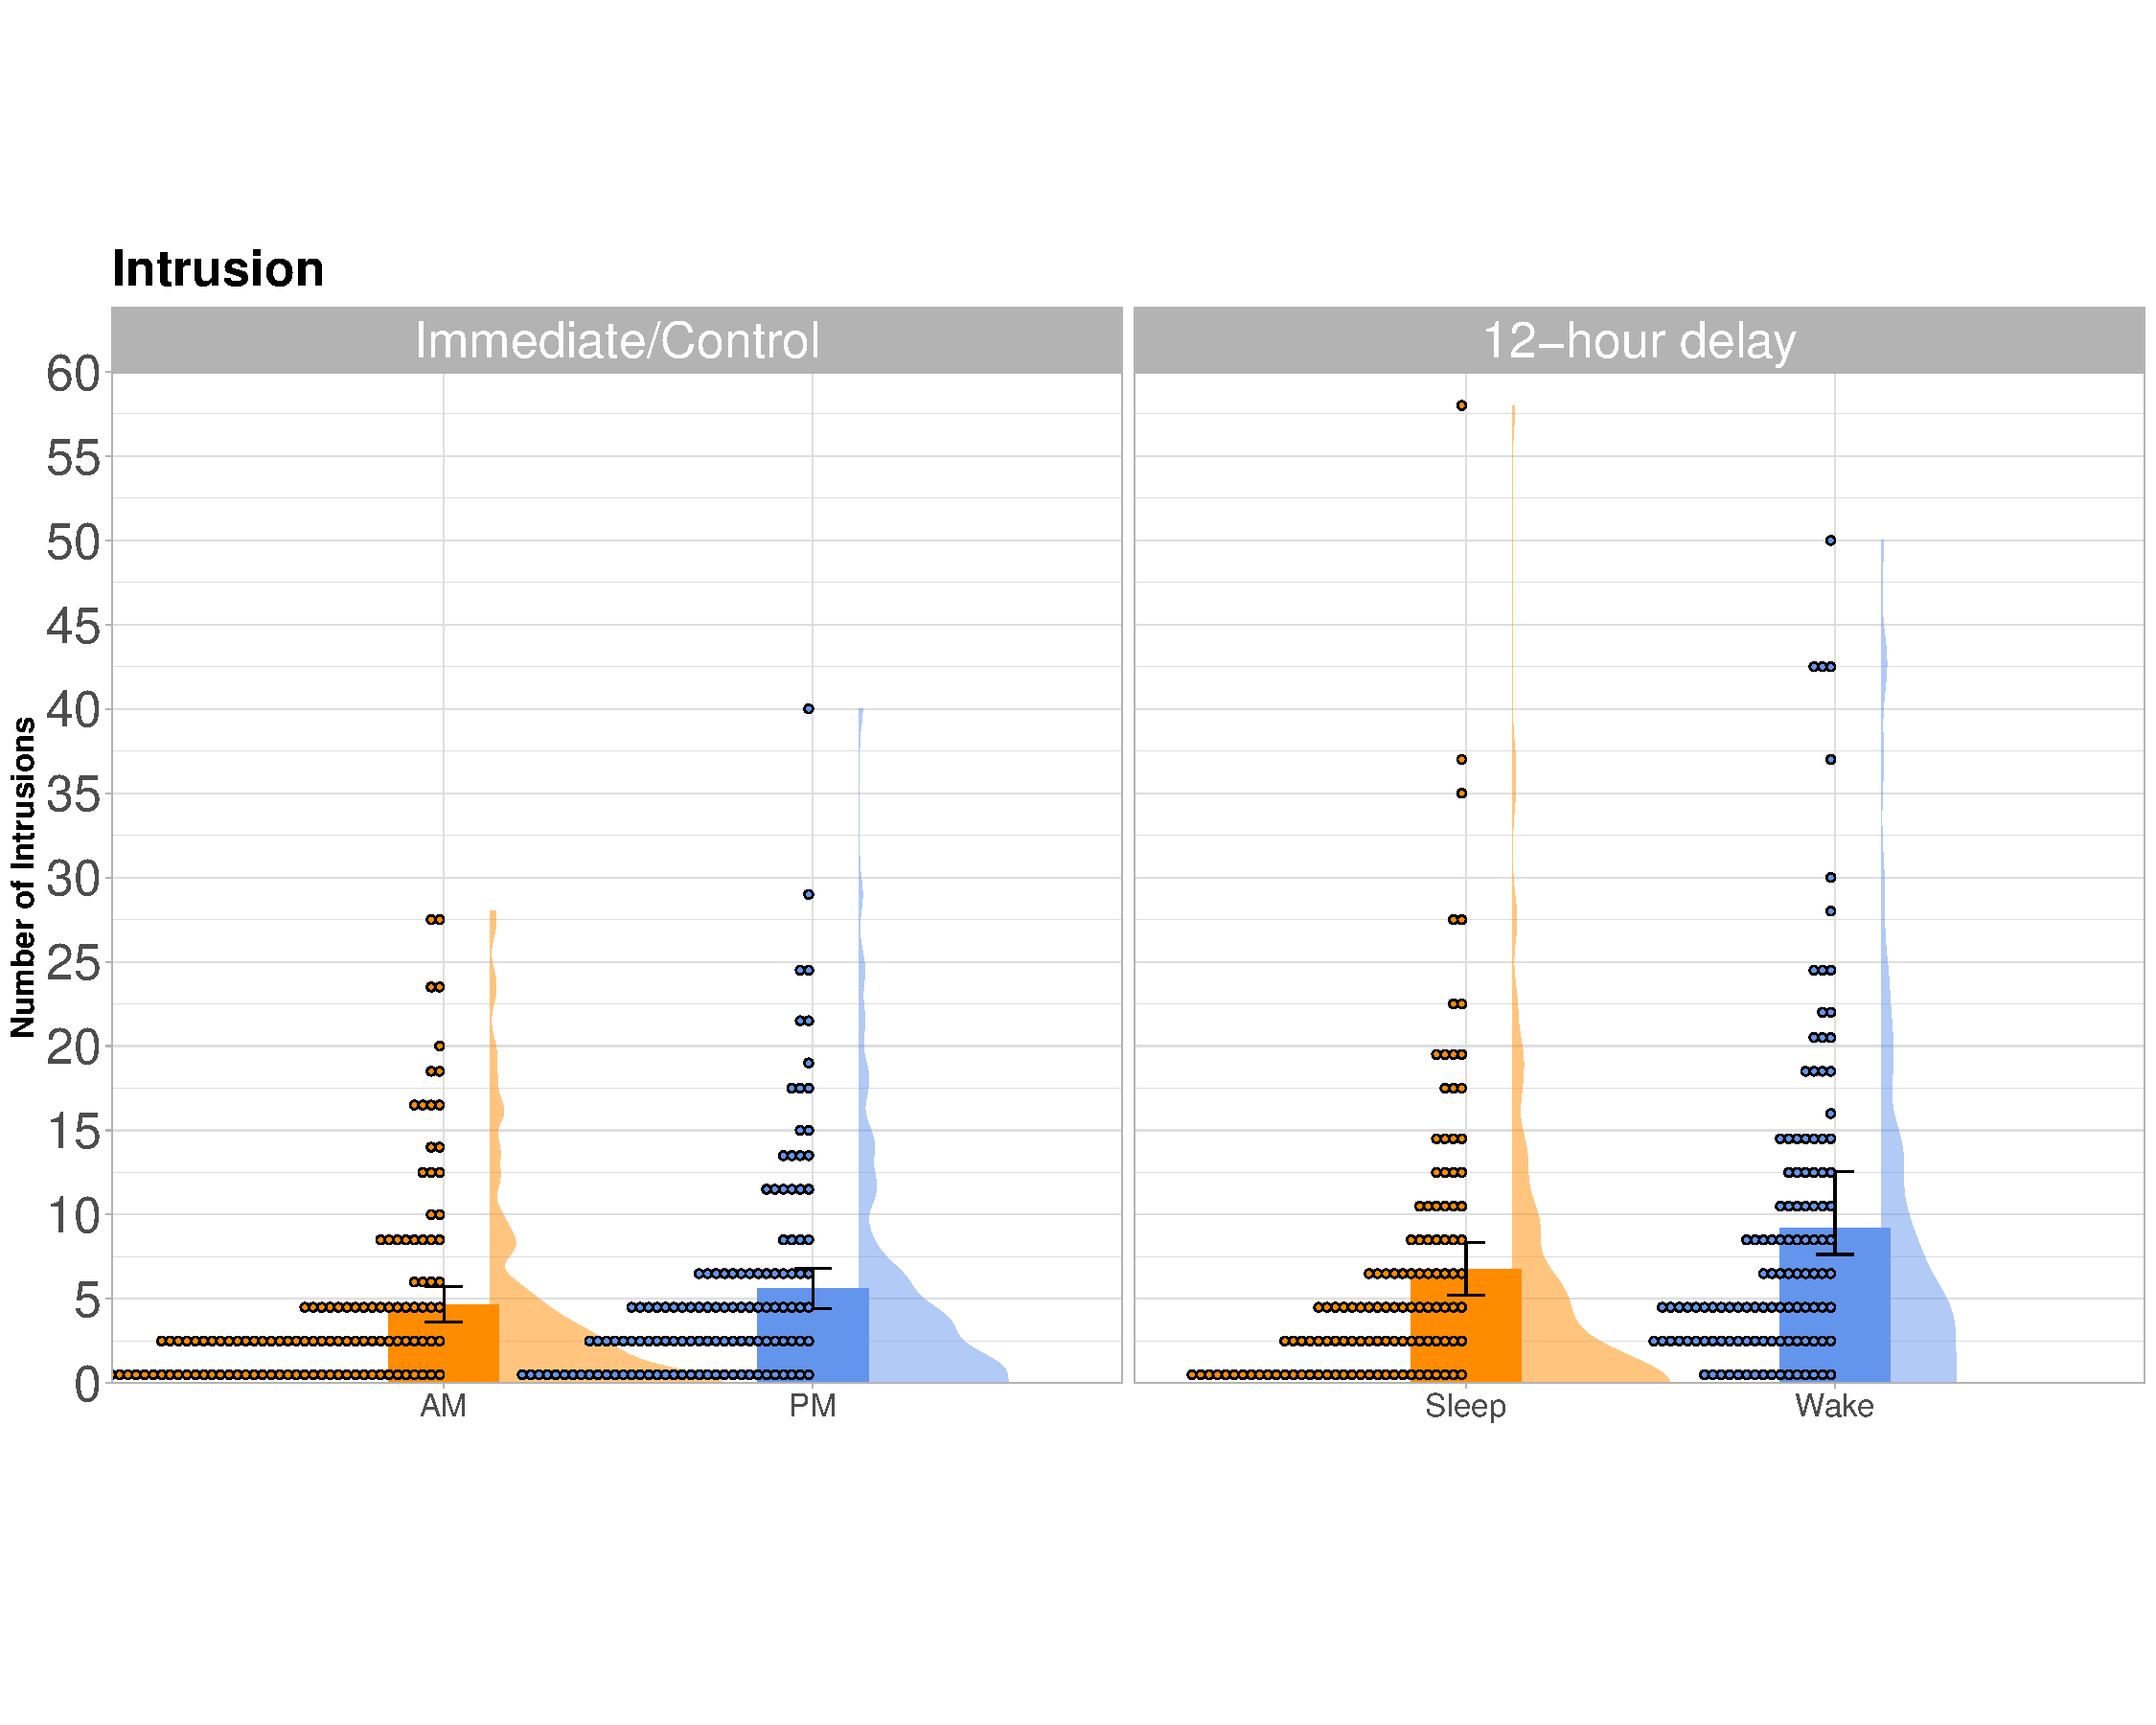
\includegraphics{Figures/intrusiongraph} 

}

\caption{Number of intrusions produced, summarised across the four groups. Each dot represents an individual participant, and the error bars represent 95\% confidence intervals.}\label{fig:intrusionfig}
\end{figure}

A 2 \(\times\) 2 Poisson regression revealed significant effects of Interval (\(\beta\) = 0.372, SE = 0.054, z = 6.845, p \textless{} \textless0.001) and Test Time (\(\beta\) = 0.185, SE = 0.056, z = 3.299, p \textless{} \textless0.001), which were qualified by a significant interaction (\(\beta\) = 0.214, SE = 0.072, z = 2.96, p = 0.003). Given this, we tested the simple effects of Test Time within the Immediate and Delay groups using the emmeans package {[}\protect\hyperlink{ref-lenth2021a}{25}{]}. Within the Immediate groups, the evening participants (M = 5.62; SD = 6.63) produced more intrusions than the morning participants (M = 4.67; SD = 5.97) (z = -3.299, p = \textless0.001). Likewise, in the Delay groups, the Wake participants, who completed free recall in the evening (M = 10.1; SD = 13.65), produced more intrusions than the Sleep participants, who completed recall in the morning (M = 6.78; SD = 8.71) (z = -8.808, p = \textless0.001). Together, our data indicate that participants who attempted free recall in the evening (vs.~morning) were more prone to intrusions, and this effect was greater in the Delay than in the Immediate groups. These unexpected findings prompted us to explore whether the number of total responses (i.e., studied + lures + intrusions) differed between morning and evening test time. Interestingly, this exploratory analysis (see section 13.1) showed no effect of Test Time. Together, these suggest that attempting free recall in the evening led to a selective increase in intrusions, but not necessarily a global increase in output bias. Finally, given that Test Time had a significant effect on intrusions, we followed our pre-registered analysis plan by adding However, neither Test Time nor their interaction is expected to be significant. If in the unlikely event that these are revealed to be significant, the number of intrusions as a numeric covariate in the 2 \(\times\) 2 mixed-effects models below.

\hypertarget{confirmatory-analysis-1.}{%
\subsection{Confirmatory analysis 1.}\label{confirmatory-analysis-1.}}

This analysis addresses our key research question:

\(\text{\underline{\#1 Does overnight sleep (vs. daytime wakefulness) influence DRM false recall?}}\)

The number of critical lures falsely recalled is summarised across groups in Figure \ref{fig:lurefig}.

\begin{figure}

{\centering 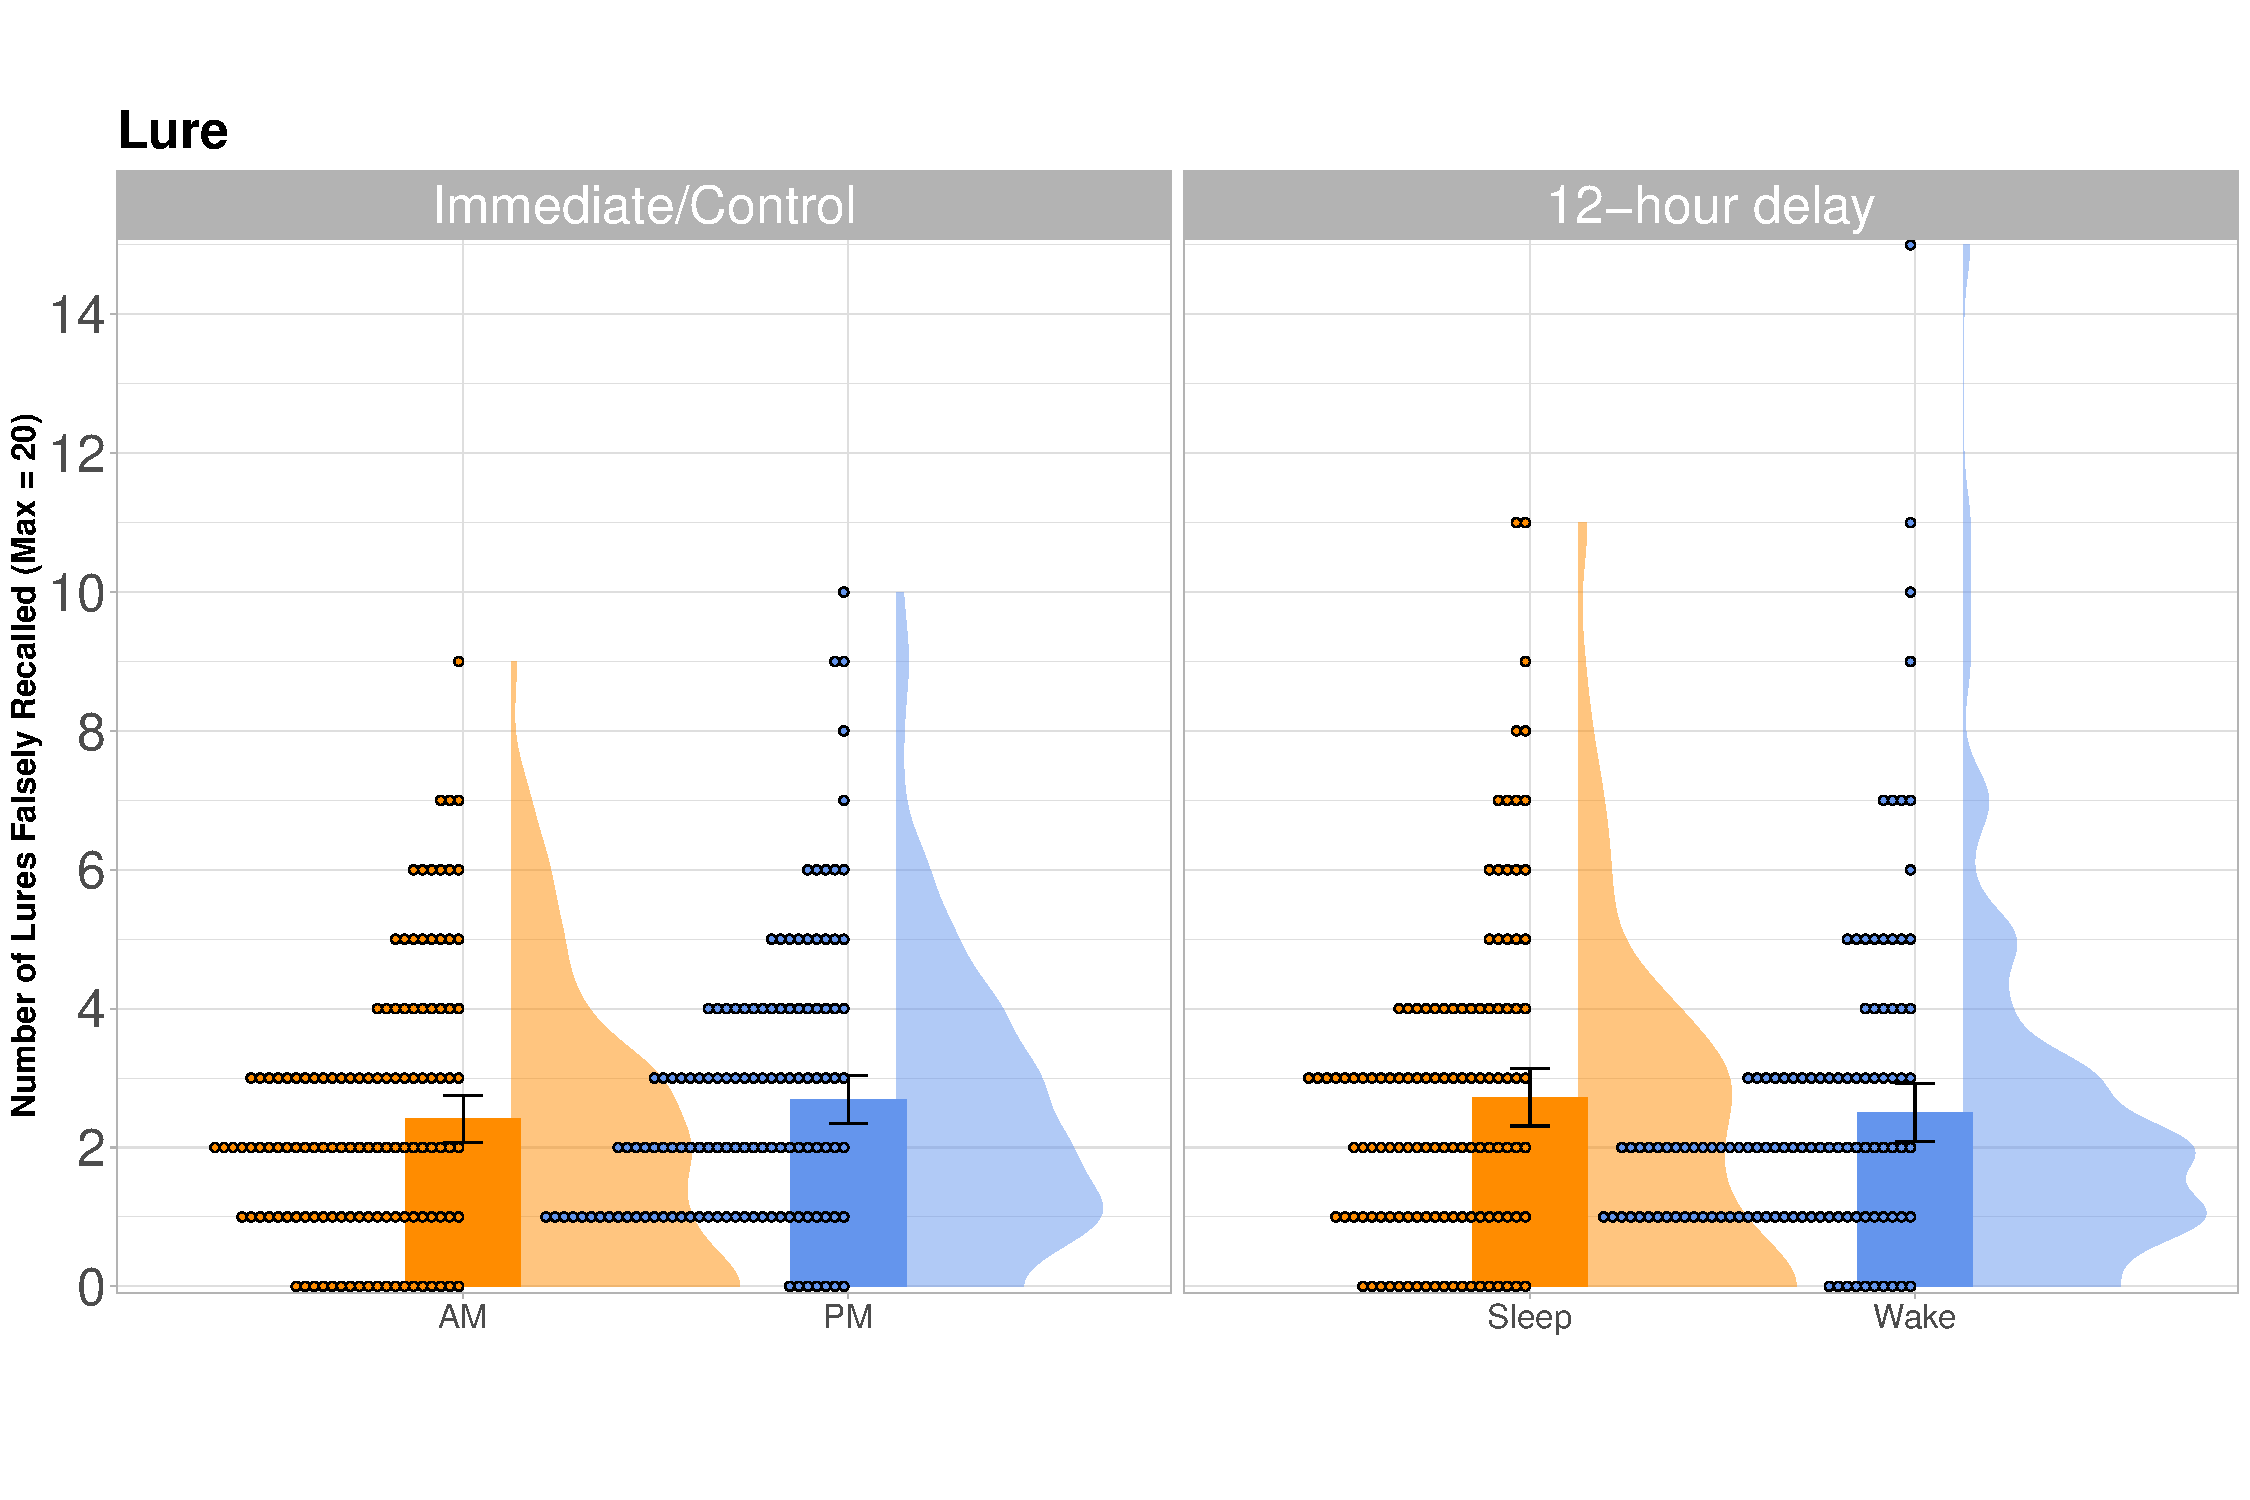
\includegraphics{Figures/luregraph} 

}

\caption{Number of critical lures falsely recalled, summarised across the four groups. Each dot represents an individual participant, and the error bars represent 95\% confidence intervals.}\label{fig:lurefig}
\end{figure}

A generalised linear mixed-effect model (GLMM) was fitted to the critical lure data on the item level (N of observations = 488` participants \(\times\) 20 critical lures).\footnote{The use of GLMM is a clear departure from prior ‘Sleep $\times$ DRM’ studies, the majority of which addressed the same research question using an independent t-test or ANOVA (e.g., Diekelmann et al., 2010; Monaghan et al., 2017; Payne et al., 2009). We explained in Appendix C why these statistical tests are usually not appropriate in the context of DRM recall and why GLMM are more advantageous.} The dependent variable was binary: whether a critical lure was recalled or not (1 vs.~0). The fixed effects were the number of intrusions a participant produced, Interval (Immediate vs.~Delay), Test Time (AM vs.~PM), and an Interval by Test Time interaction. Interval and Test Time were coded using sum contrasts {[}\protect\hyperlink{ref-barr2019a}{26}{]}. The random-effect structure was determined by the ``buildmer'' package {[}\protect\hyperlink{ref-voeten2021a}{27}{]}, which automatically found the maximal model that was capable of converging using backward elimination (with the ``bobyqa'' optimiser). This means that model selection started from the maximal model, as justified by the experimental design {[}\protect\hyperlink{ref-barr2013a}{28}{]}. The model we reported and based our interpretation on was the most maximal model that was capable of converging (see the upper half of Table \ref{tab:table4} for the final random-effect structure and model output).

\begin{table}[H]

\caption{\label{tab:table4}Outputs from confirmatory generalised mixed-effect models examining the effects of Intrusions, Interval, and Test Time in false and veridical recall.}
\centering
\begin{tabular}[t]{lllll}
\toprule
\multicolumn{5}{c}{\textbf{False (lure) recall}} \\
\cmidrule(l{3pt}r{3pt}){1-5}
\multicolumn{5}{l}{Random-effect structure: (Intrusions | Participant.ID) + (1 | Lure)} \\
\cmidrule(l{3pt}r{3pt}){1-5}
\em{} & \em{Estimate} & \em{SE} & \em{z} & \em{p}\\
Intercept & -2.328 & 0.11 & -21.254 & <.001*\\
Intrusions & 0.034 & 0.006 & 5.487 & <.001*\\
Interval (Immediate vs. Delay) & 0.039 & 0.042 & 0.943 & .346\\
Test Time (AM vs. PM) & 0.035 & 0.041 & 0.85 & .395\\
\addlinespace
Interval x Test Time & -0.084 & 0.041 & -2.046 & .041*\\
\bottomrule
\end{tabular}
\end{table}

\begin{table}[H]
\centering
\begin{tabular}{lllll}
\toprule
\multicolumn{5}{c}{\textbf{Veridical (studied word) recall}} \\
\cmidrule(l{3pt}r{3pt}){1-5}
\multicolumn{5}{l}{Random-effect structure: (Intrusions | Participant.ID) + (Interval | Studied.Item)} \\
\cmidrule(l{3pt}r{3pt}){1-5}
\em{} & \em{Estimate} & \em{SE} & \em{z} & \em{p}\\
Intercept & -2.373 & 0.075 & -31.705 & <.001*\\
Intrusions & -0.007 & 0.005 & -1.372 & .17\\
Interval (Immediate vs. Delay) & 0.307 & 0.04 & 7.721 & <.001*\\
Test Time (AM vs. PM) & 0.026 & 0.037 & 0.691 & .489\\
\addlinespace
Interval x Test Time & -0.124 & 0.037 & -3.325 & <.001*\\
\bottomrule
\end{tabular}
\end{table}

The number of intrusions had a significant effect on lure recall, such that participants who produced more intrusions tended to recall more critical lures (z = 5.487, p \textless{} \textless.001). There were no main effects of Interval or Test Time (zs \textless{} 0.95, ps \textgreater{} .34), but there was a significant Interval by Test Time interaction (z = -2.046, p \textless{} .041). Following our pre-registered analysis plan, we proceeded to test the simple effects of Test Time within the Immediate and Delay groups, using the emmeans package {[}\protect\hyperlink{ref-lenth2021a}{25}{]} in R. Among the Immediate groups, there was no significant difference in lure recall between the AM-control and PM-control participants (\(\beta\) = -0.098, SE = 0.114, z = -0.859, p = .39). However, among the Delay groups, there was a significant difference (\(\beta\) = 0.239, SE = 0.119, z = 2, p = .045) such that the Sleep participants (M = 2.72, SD = 2.3) reported more critical lures than the Wake participants (M = 2.51, SD = 2.32).

\hypertarget{box-1}{%
\subsection*{Box 1}\label{box-1}}
\addcontentsline{toc}{subsection}{Box 1}

\emph{R codes for Confirmatory Analysis 1}

\begin{Shaded}
\begin{Highlighting}[]
\FunctionTok{contrasts}\NormalTok{(FalseRecall}\SpecialCharTok{$}\NormalTok{Interval) }\OtherTok{\textless{}{-}} \FunctionTok{contr.sum}\NormalTok{(}\DecValTok{2}\NormalTok{)  }\CommentTok{\#sum contrast for interval}
\FunctionTok{contrasts}\NormalTok{(FalseRecall}\SpecialCharTok{$}\NormalTok{Test\_Time) }\OtherTok{\textless{}{-}} \FunctionTok{contr.sum}\NormalTok{(}\DecValTok{2}\NormalTok{) }\CommentTok{\#sum contrast for test time}
\FunctionTok{library}\NormalTok{(lme4) }
\FunctionTok{library}\NormalTok{(buildmer) }
\CommentTok{\# 2 x 2 GLMM}
\NormalTok{FalseRecallModel }\OtherTok{\textless{}{-}} \FunctionTok{buildmer}\NormalTok{(Recalled }\SpecialCharTok{\textasciitilde{}}\NormalTok{ Interval }\SpecialCharTok{*}\NormalTok{ Test\_Time }\SpecialCharTok{+}\NormalTok{ (}\DecValTok{1} \SpecialCharTok{|}\NormalTok{ Participant) }\SpecialCharTok{+} 
\NormalTok{                    (Interval }\SpecialCharTok{*}\NormalTok{ Test\_Time }\SpecialCharTok{|}\NormalTok{ Item), }\AttributeTok{data =}\NormalTok{ FalseRecall, }\AttributeTok{family =} 
                    \StringTok{"binomial"}\NormalTok{,}\AttributeTok{buildmerControl =} \FunctionTok{buildmerControl}\NormalTok{(}\AttributeTok{direction=}\StringTok{\textquotesingle{}backward\textquotesingle{}}\NormalTok{, }
                    \AttributeTok{args =} \FunctionTok{list}\NormalTok{(}\AttributeTok{control=}\FunctionTok{glmerControl}\NormalTok{(}\AttributeTok{optimizer=}\StringTok{"bobyqa"}\NormalTok{))))}
\CommentTok{\# Obtain the simple{-}effects of Test Test within the Immediate and Delay groups}
\FunctionTok{library}\NormalTok{(emmeans)}
\FunctionTok{emmeans}\NormalTok{(FalseRecallModel, pairwise }\SpecialCharTok{\textasciitilde{}}\NormalTok{ Test\_Time }\SpecialCharTok{|}\NormalTok{ Interval)}
\end{Highlighting}
\end{Shaded}

\hypertarget{confirmatory-analysis-2.}{%
\subsection{Confirmatory analysis 2.}\label{confirmatory-analysis-2.}}

This analysis addresses the secondary question:

\(\text{\underline{\#2 Does overnight sleep (vs. daytime wakefulness) increase veridical recall of the studied list words?}}\)

Figure \ref{fig:studiedfig} summarises the number of studied list words correctly recalled across groups.

\begin{figure}

{\centering 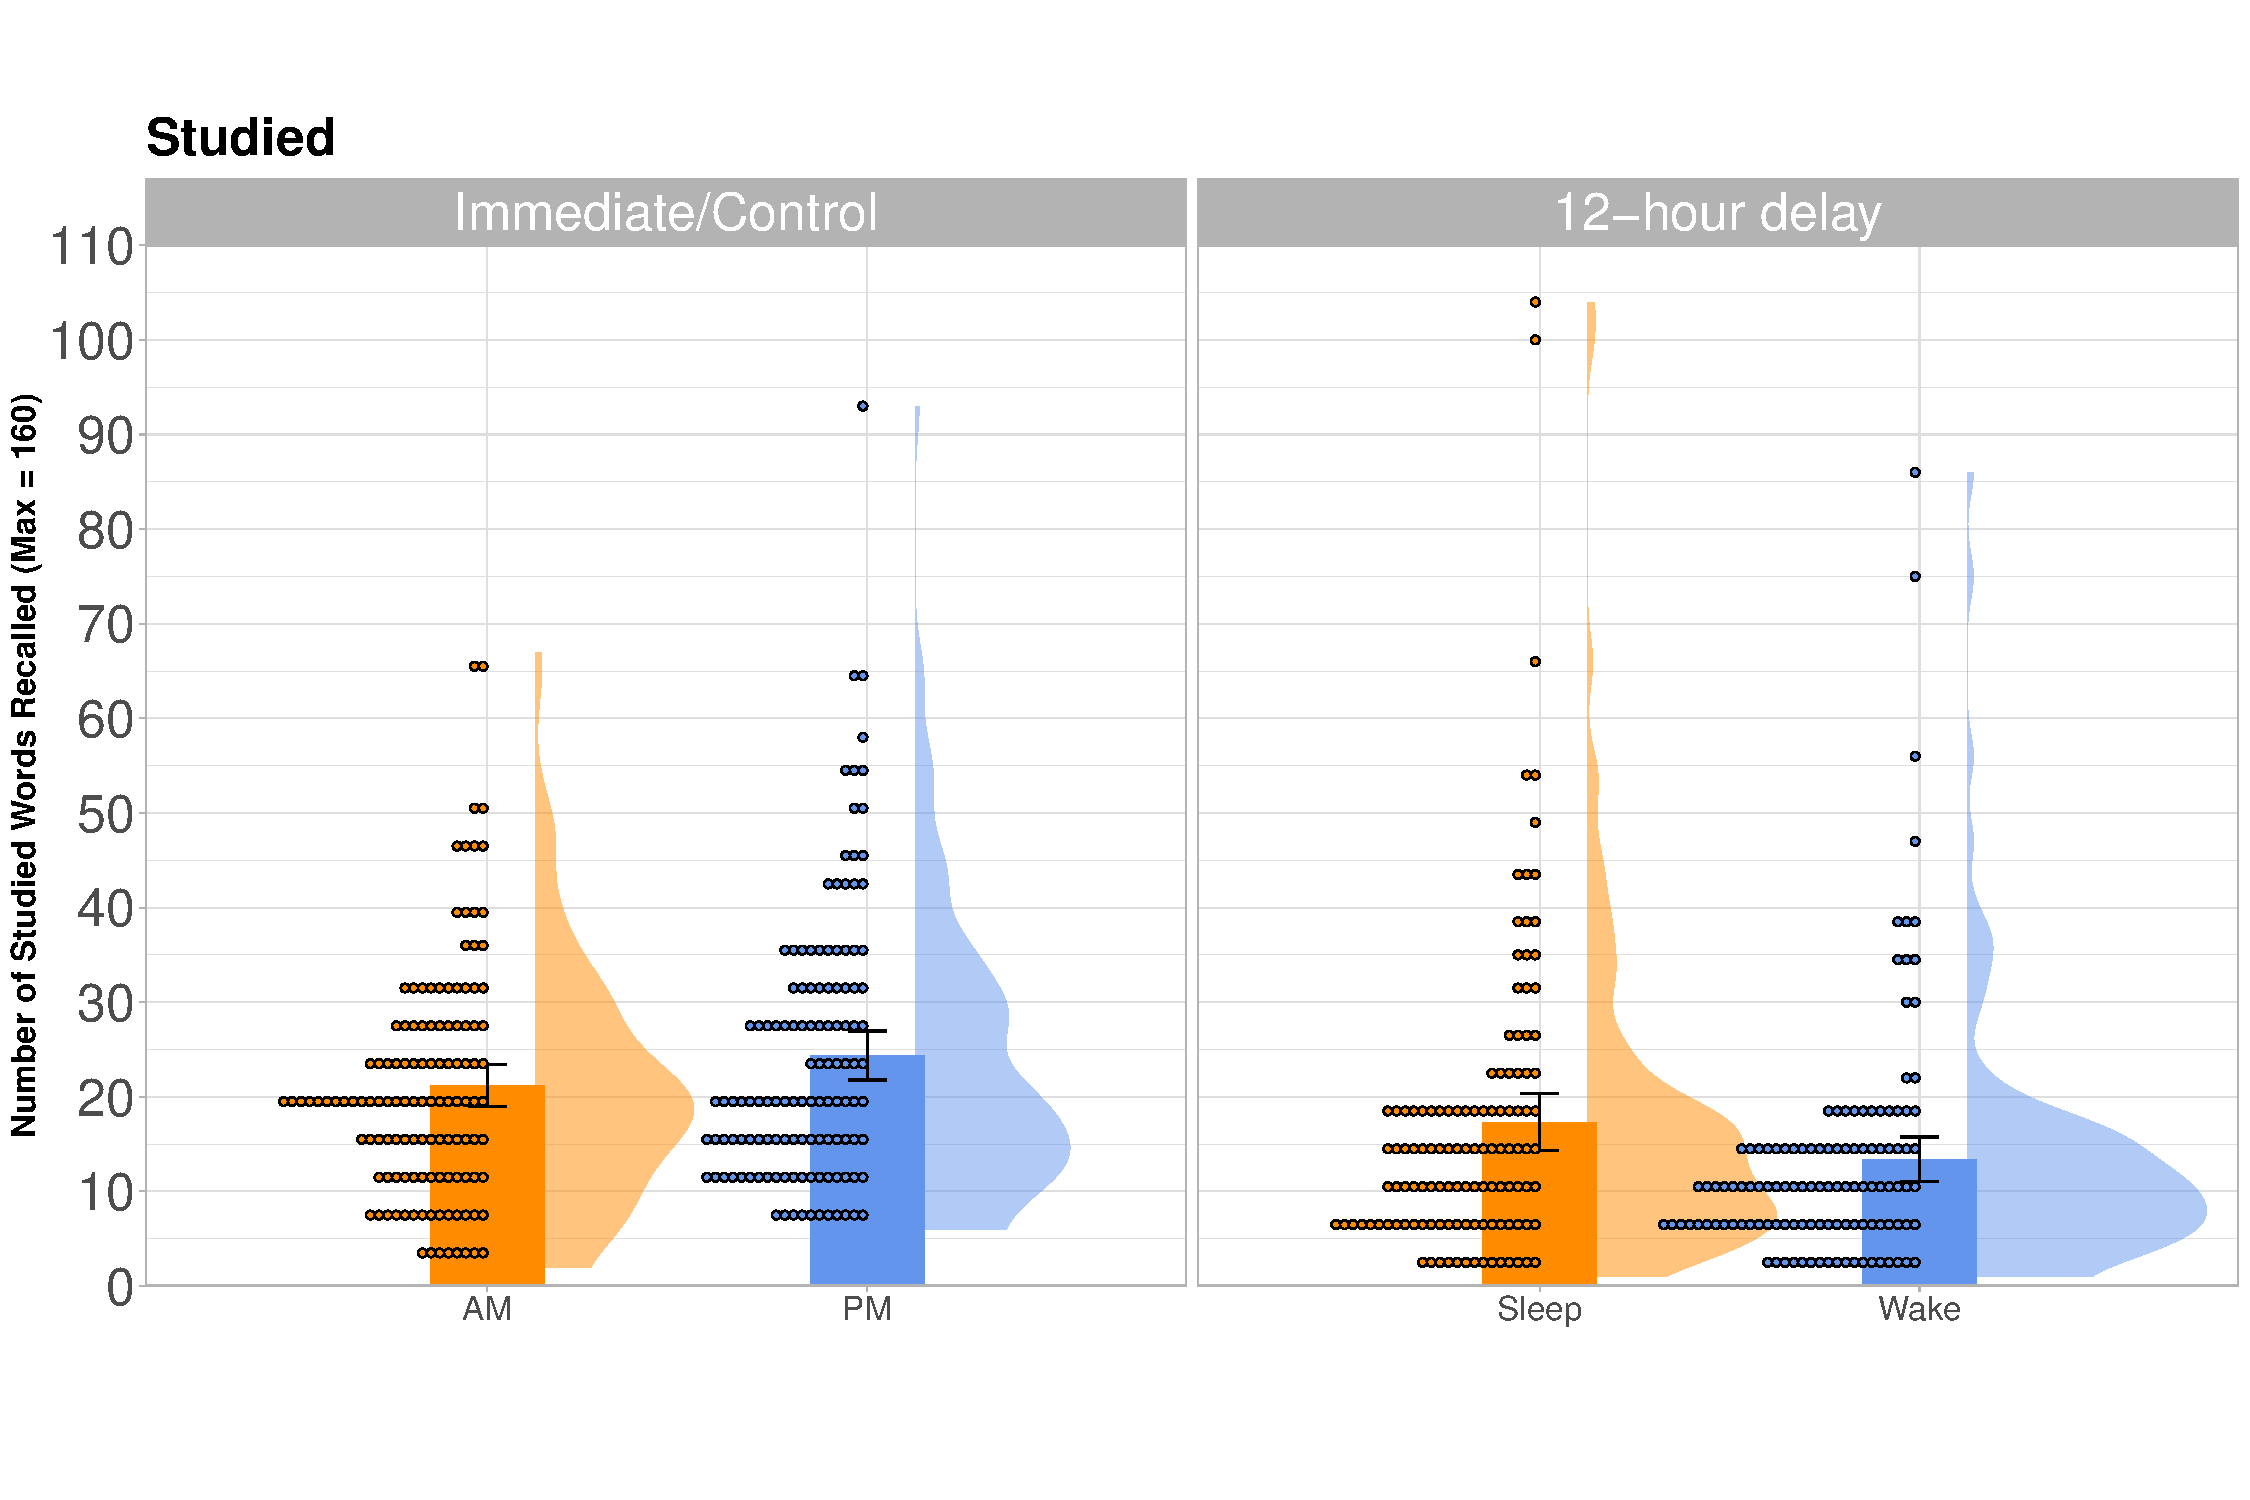
\includegraphics{Figures/studiedgraph} 

}

\caption{Number of studied list words correctly recalled, summarised across the four groups. Each dot represents an individual participant, and the error bars represent 95\% confidence intervals.}\label{fig:studiedfig}
\end{figure}

We fitted a GLMM to the veridical recall dataset (N of observations = 488 participants \(\times\) 160 studied words). The dependent variable was whether a studied word was recalled or not. The fixed effects were the the number of intrusions a participant produced, Interval (Immediate vs.~Delay), Test Time (AM vs.~PM), and an Interval by Test Time interaction. The coding scheme and computation procedure were the same as in the previous analysis. The model output and its random-effect structure are available in the lower half of Table \ref{tab:table4}. There were no significant effects of intrusions (z = -1.372, p = .17) or Test Time (z = 0.691, p = .489). However, there was a main effect of Interval (z = 7.721, p \textless.001) such that participants in the Delay groups recalled significantly fewer studied words (M = 15.37, SD = 14.97) than those in the Immediate groups (M = 22.77, SD = 13.59), indicating time-dependent memory decay. Importantly, there was a significant Interval by Test Time interaction (z = -3.325, p \textless.001*), so we broke it down with the emmeans package as pre-registered. Within the Immediate groups, the evening participants (M = 24.36, SD = 14.6) recalled more studied words than the morning participants (M = 21.18, SD = 12.36), although this was not statistically significant (\(\beta\) = -0.196, SE = 0.104, z = -1.88, p = .06). Within the Delay groups, there was a main effect of Test Time (\(\beta\) = 0.299, SE = 0.107, z = 2.797, p = .0052), such that the Sleep participants (M = 17.32, SD = 16.59) outperformed their Wake counterparts (M = 13.41, SD = 12.93). Together, these support the well-established findings that sleep is typically beneficial to the retention of newly encoded declarative memories.

\hypertarget{complementary-bayesian-analysis}{%
\subsubsection{Complementary Bayesian analysis}\label{complementary-bayesian-analysis}}

Although our inference was based on a frequentist approach, we pre-registered to use a Bayesian analysis to complement and test the strength of our results.

Bayes Factors were computed for (1) the Interval \(\times\) Test Time interaction in the false and veridical mixed-effect models above, and for the simple effects of Test Time within the (2) Immediate and (3) Delay groups. Following the procedures in Gilbert et al. {[}\protect\hyperlink{ref-gilbert2018a}{29}{]}, a Bayes Factor was computed using the Bayesian Information Criterion (BIC) approximation from two competing GLMMs. For instance, in computing the Bayes Factor for the Interval \(\times\) Test Time interaction, two models were needed: An alternative model containing the full fixed-effects structure (Intrusions + Interval + Test Time + Interval \(\times\) Test Time), and a null model lacking the interaction.\footnote{To obtain the Bayes Factor for the simple effects of Test Time, the alternative model will contain Test Time as the sole fixed effect while the null model will contain no fixed effects.} To estimate the Bayes Factor, we used the formula e \(e{\Delta BIC_{10}/2}\), where \(\Delta BIC_{10}\) is the BIC for the null model minus the BIC for the alternative model {[}\protect\hyperlink{ref-masson2011a}{30}--\protect\hyperlink{ref-wagenmakers2007a}{32}{]}. This produces a Bayes Factor\(_{10}\), which was interpreted with reference to Lee and Wagenmakers' {[}\protect\hyperlink{ref-lee2014a}{33}{]} heuristics. The current BIC approximation method has the advantage of being a straightforward solution for mixed-effects models; however, its usage remains controversial as it is known to favour the simpler model (i.e., the null hypothesis; {[}\protect\hyperlink{ref-lindelov2018a}{31},\protect\hyperlink{ref-vandekerckhove2014a}{\textbf{vandekerckhove2014a?}},\protect\hyperlink{ref-weakliem1999a}{\textbf{weakliem1999a?}}{]}). Table \ref{tab:table5} summarises the Bayes Factors derived from our mixed-effects models.

\begin{table}[H]

\caption{\label{tab:table5}Bayes Factors for the Interval x Test Time interactions and the simple effects of Test Time in the lure and veridical recall data.}
\centering
\begin{tabular}[t]{ll}
\toprule
Effects & Bayes Factor 10\\
\midrule
\em{False (lure) recall} & \em{}\\
Interval x Test Time & 2e-05\\
Test Time in Immediate groups & 0.5\\
Test Time in Delay groups & 0.5\\
\em{Veridical (studied word) recall} & \em{}\\
\addlinespace
Interval x Test Time & 29122042\\
Test Time in Immediate groups & 0.00127\\
Test Time in Delay groups & 0.01763\\
\bottomrule
\end{tabular}
\end{table}

Surprisingly, all the Bayes Factors, except for the Interval \(\times\) Test Time interaction in the studied word model, were below 0.1. These, according to Lee and Wagenmakers {[}\protect\hyperlink{ref-lee2014a}{33}{]}, can be taken as extreme evidence for the null hypotheses. In other words, there is a discrepancy between our frequentist and Bayesian analyses. We stress that this Bayesian analysis is complementary in nature and our primary test of significance remains the frequentist test.

\hypertarget{results-of-exploratory-analyses}{%
\section{Results of Exploratory Analyses}\label{results-of-exploratory-analyses}}

In this section, we present the results of four exploratory analyses, which explored {[}1{]} the number of total responses (i.e., studied + lure + intrusions) across groups, {[}2{]} whether the effect of sleep on lure recall is modulated by veridical recall, as suggested by Diekelmann et al. {[}\protect\hyperlink{ref-diekelmann2010a}{34}{]}, {[}3{]} the extent to which a lure being produced is predicted by its corresponding list items being recalled, and {[}4{]} the semantic distance between intrusions and critical lures.

\hypertarget{number-of-total-responses}{%
\subsection{Number of total responses}\label{number-of-total-responses}}

In light of the finding that participants who completed free recall in the evening (vs.~morning) produced more intrusions, we asked whether this was driven by these participants having a greater tendency to put down more responses generally. To test this, we calculated the number of total responses by each participant (i.e., studied + lures + intrusions), which is summarised across groups in Figure 5.

Unlike the intrusion data which had an overall mean of 6.8 and a minimum of 0, the number of total responses had a mean of 28.5 and a minimum of 2, suggesting that it is better to consider total responses as continuous, as opposed to count, data. As such, we used a 2 \(\times\) 2 between-participant ANOVA to test for the effects of Interval and Test Time on the number of total responses, which was log-transformed to give a more normal distribution. The ANOVA revealed a main effect of Interval {[}F(1, 484) = 21.35, p \textless.001{]}, such that participants in the Immediate groups (M = 30.5, SD = 15) gave more responses than those in the Delay groups (M = 26.4, SD = 20.1). This pattern is consistent with the confirmatory analysis on the studied list words. However, importantly, there was no significant effect of Test Time {[}F(1, 484) = 1.68, p = .196{]}, and the Interval by Test Time interaction was also non-significant {[}F(1, 484) = 2.39, p = .123{]}. Together with the intrusion data, this exploratory analysis suggests that attempting free recall in the evening led to a selective increase in intrusions but not necessarily an increase in general response bias.

\hypertarget{is-the-effect-of-sleep-on-false-recall-modulated-by-veridical-memory}{%
\subsection{Is the effect of sleep on false recall modulated by veridical memory?}\label{is-the-effect-of-sleep-on-false-recall-modulated-by-veridical-memory}}

In 36 participants (18 Sleep and 18 Wake), Diekelmann et al. {[}\protect\hyperlink{ref-diekelmann2010a}{34}{]} found that the effect of sleep on DRM false recall was modulated by veridical recall. In their analysis, they performed a post-hoc median split on adjusted veridical recall (i.e., correct recall minus intrusions), separating their participants as either high or low performers. They reported that participants in the Sleep (vs.~Wake) group falsely recalled more lures, but only if they were low performers. This finding, as far as we can see, has yet to be replicated, so we explored whether it could be observed in our data, which is more well-suited to test for individual differences given our large sample size.

In this exploratory analysis, we followed Diekelmann et al. {[}\protect\hyperlink{ref-diekelmann2010a}{34}{]} by focusing on the Delay groups\footnote{Note that Diekelmann et al. (2010) did not have Immediate/Control groups.} and by performing a median split on our sample's adjusted veridical recall (Median = 5), classifying our participants as either high (\textgreater5; N = 117) or low ( \(\leq\) 5; N = 123) performers. We followed the analysis approach of Diekelmann et al. {[}\protect\hyperlink{ref-diekelmann2010a}{34}{]}, but since the number of critical lures a participant produced is count data, we used a 2 (Group: Sleep vs.~Wake) \(\times\) 2 (Adjusted veridical recall: High vs.~Low Performers) Poisson regression, instead of an ANOVA. This analysis showed no main effect of Group (\(\beta\) = -0.052, z = -0.494, p = .621) but a main effect of Adjusted veridical recall (\(\beta\) = -0.438, z = -3.766, p \textless{} .001), such that high performers (M = 3.17, SD = 2.71) tended to falsely recall more critical lures than low performers (M = 2.09, SD = 1.68) ({[}\protect\hyperlink{ref-thapar2001a}{\textbf{thapar2001a?}},\protect\hyperlink{ref-toglia1999}{\textbf{toglia1999?}}{]}, but see {[}\protect\hyperlink{ref-roediger2001a}{21},\protect\hyperlink{ref-stadler1999a}{35},\protect\hyperlink{ref-cann2011a}{\textbf{cann2011a?}}{]}). Furthermore, importantly, the interaction between Group and Adjusted veridical recall was not significant (\(\beta\) = 0.049, z = 0.30, p = .763). Despite this, we followed Diekelmann et al. {[}\protect\hyperlink{ref-diekelmann2010a}{34}{]} by comparing low performers in the Sleep and Wake groups. Contrary to their findings, emmeans showed that our low performers in both groups recalled essentially the same number of critical lures (MSleep = 2.09, SDSleep = 1.63 vs.~Mwake = 2.09, SDWake = 1.74; \(\beta\) = 0.133, z = 0.021, p = .982). In other words, this exploratory analysis found no evidence that the effect of sleep on false recall was modulated by veridical memory, casting doubt over the robustness and reliability of Diekelmann et al.'s {[}\protect\hyperlink{ref-diekelmann2010a}{34}{]} findings.

\hypertarget{the-relationship-between-lure-and-veridical-recall-on-a-list-level}{%
\subsection{The relationship between lure and veridical recall on a list level}\label{the-relationship-between-lure-and-veridical-recall-on-a-list-level}}

Here, we asked whether recall probability of a lure (e.g., doctor) is predicted by the number of corresponding list items being recalled (e.g., nurse, hospital, sick), and if it does, whether it differs between the Sleep and Wake groups. These questions help shed light on the degree to which sleep increases lure recall via processes such as retrieval-induced generalisation\footnote{Retrieval-induced generalisation: Retrieval of one word cueing retrieval of a related word (e.g., Berens \& Bird, 2017)} or gist abstraction\footnote{Gist abstraction: Extraction of the central or essential meaning of learned information}, as these processes may predict a different degree of interdependence between lure and veridical recall. If sleep (vs.~wake) promoted retrieval-induced generalisation, lure and veridical recall should become more strongly correlated with each other after sleep, because better veridical recall for a set of studied words may generalise to the corresponding critical lure (or vice versa). On the other hand, if sleep (vs.~wake) promoted gist abstraction, lure recall may become less related to memories for the corresponding list items, because theories of gist abstraction such as iOtA may predict that sleep would selectively boost the overlapping gist memory (i.e., the lure) but not necessarily the specific studied words.

In this exploratory analysis, we first calculated a participant's number of correct recalls per DRM wordlist (Range = 0 - 8) and used this to predict recall of the corresponding critical lure in a generalised mixed-effect model, which had Number of intrusions, Number of correct recall per list, Interval (Immediate vs.~Delay), Test Time (AM vs.~PM), and an interaction of the latter three as the fixed effects. Interval and Test Time were effect coded, and the random-effect structures contained a by-participant intercept only, as prescribed by the buildmer package. The model output is summarised in Table \ref{tab:table6}.

\begin{table}[H]

\caption{\label{tab:table6}Outputs from the exploratory generalised mixed-effect model examining the effects of intrusions, correct recall per list, Interval (Immediate vs. Delay), and Test Time (Sleep vs. Wake) in false recall.}
\centering
\begin{tabular}[t]{lllll}
\toprule
\textbf{Fixed effects} & \textbf{Estimate} & \textbf{SE} & \textbf{z} & \textbf{p}\\
\midrule
Intercept & -3.543 & 0.092 & -38.6 & <.001\\
Intrusions & 0.034 & 0.006 & 6.011 & <.001\\
Correct recall/list & 0.799 & 0.025 & 31.848 & <.001\\
Test Time & 0.092 & 0.07 & 1.319 & .187\\
Interval & 0.039 & 0.07 & 0.551 & .582\\
\addlinespace
Correct recall/list x Test Time & -0.062 & 0.022 & -2.778 & .00548\\
Correct recall/list x Interval & -0.127 & 0.022 & -5.702 & <.001\\
Interval x Test Time & -0.095 & 0.069 & -1.372 & .17\\
Correct recall/list x Interval x Test Time & 0.062 & 0.022 & 2.798 & .00514\\
\bottomrule
\end{tabular}
\end{table}

Given the significant three-way interaction, we broke it down by computing two additional GLMMs, one within the Immediate and another within the Delay group. These models had Number of intrusions, Number of correct recall per list, Test Time (AM vs.~PM), and an interaction of the latter two as the fixed effects. Table \ref{tab:table7} summarises the model outputs.

\begin{table}[H]

\caption{\label{tab:table7}Outputs from the exploratory generalised mixed effect models examining the effects of Intrusions, Correct recall per list, and Test Time (Sleep vs. Wake) in false recall.}
\centering
\begin{tabular}[t]{lllllllll}
\toprule
\multicolumn{1}{c}{\textbf{}} & \multicolumn{4}{c}{\textbf{Immediate}} & \multicolumn{4}{c}{\textbf{Delay}} \\
\cmidrule(l{3pt}r{3pt}){2-5} \cmidrule(l{3pt}r{3pt}){6-9}
\textbf{Fixed effects} & \textbf{Estimate} & \textbf{SE} & \textbf{z} & \textbf{p} & \textbf{Estimate} & \textbf{SE} & \textbf{z} & \textbf{p}\\
\midrule
Intercept & -3.681 & 0.153 & -24.109 & <.001* & -3.544 & 0.136 & -26.104 & <.001*\\
Intrusions & 0.07 & 0.01 & 6.854 & <.001* & 0.023 & 0.007 & 3.243 & .001*\\
Correct recall/list & 0.656 & 0.03 & 22.033 & <.001* & 0.95 & 0.041 & 23.121 & <.001*\\
Test Time & 0.022 & 0.09 & 0.245 & .807 & 0.163 & 0.104 & 1.571 & .116\\
Correct recall/list x Test Time & -0.001 & 0.026 & -0.037 & .971 & -0.125 & 0.036 & -3.471 & <.001*\\
\bottomrule
\end{tabular}
\end{table}

Across the Immediate and Delay groups, the number of intrusions and correct recall per list both had a main effect (ps \(\leq\) .001) such that they were positively correlated with lure recall. However, the effect of Test Time was not significant in either group (ps \textgreater{} .11). Finally, for the Correct recall per list \(\times\) Test Time interaction, it was significant in the Delay (z = -3.504, p \textless{} .001) but not the Immediate groups (z = -0.037, p = .971). To interpret the former, we used the R package, effects {[}\protect\hyperlink{ref-fox2022a}{\textbf{fox2022a?}}{]}, to visualise it (see Figure \ref{fig:delayfig}A) and plotted lure recall probability against veridical recall on a participant level (see Figure \ref{fig:delayfig}B).

\begin{figure}

{\centering 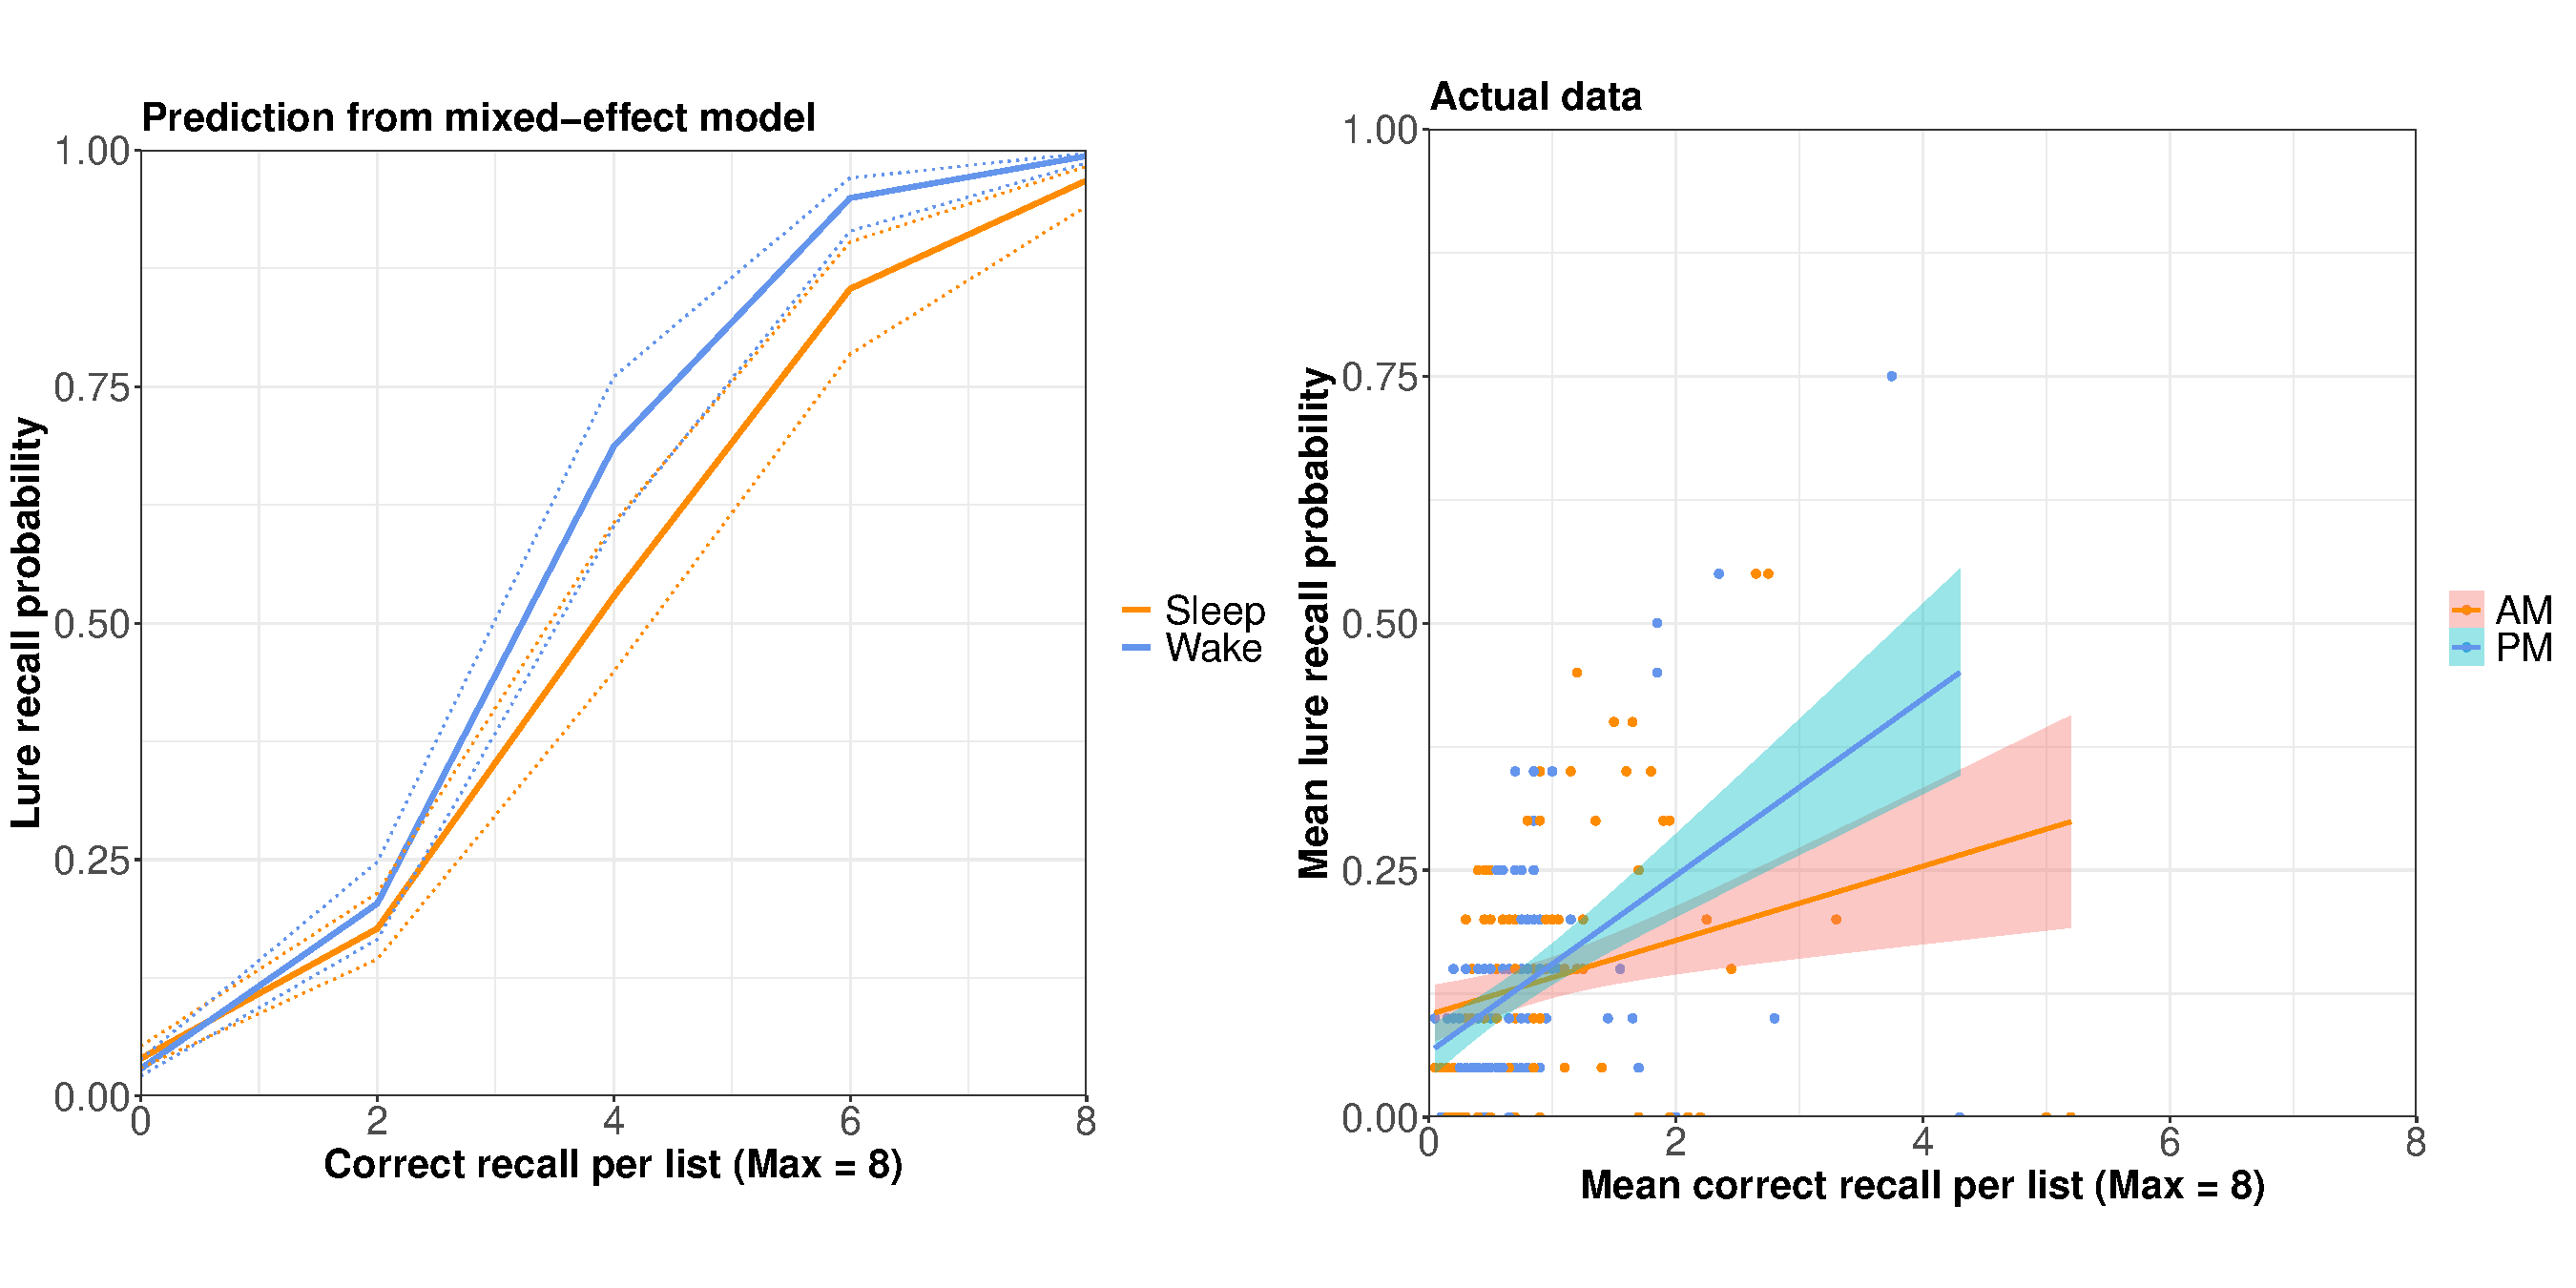
\includegraphics{Figures/delaygraph} 

}

\caption{(A) Prediction from generalised mixed-effect model on the combined effects of correct recall/list and group (sleep vs. wake) on false recall (B) Correlation between mean lure and studied word recall in the Sleep and Wake groups. Each dot represents an individual participant. Dotted lines/shaded areas represent 95\% confidence intervals.}\label{fig:delayfig}
\end{figure}

In line with the previous exploratory analysis on adjusted veridical recall, we found that when a participant recalled more studied items from a DRM wordlist, they were also more likely to recall the corresponding critical lure, suggesting some kind of retrieval-induced generalisation; importantly, however, this effect was weaker in the Sleep than the Wake participants. This finding is striking, especially in light of our confirmatory findings that overall, the Sleep participants produced more critical lures (with intrusions controlled for) and more studied list items than the Wake participants. What this exploratory analysis suggests is that after sleep (vs.~wakefulness), whether a lure was recalled may be less reliant on the retrieval of its corresponding studied items, potentially hinting that sleep may affect DRM false memory primarily via some kinds of gist abstraction process.

\hypertarget{semantic-distance-between-intrusions-and-critical-lures}{%
\subsection{Semantic distance between intrusions and critical lures}\label{semantic-distance-between-intrusions-and-critical-lures}}

As per the DRM literature, responses that were neither the studied list words nor the critical lures were classified as (non-critical) intrusions. For instance, our participants studied nurse, sick, lawyer, medicine, health, hospital, dentist, and physician, with doctor as the critical lure. Responses such as clinic and coconut would both be considered intrusions, but clearly, clinic is semantically more related to the studied list words than coconut. In other words, there is much diversity within the intrusion data. Here, we explored whether our four groups differed in terms of the semantic distance between intrusions and critical lures, as indexed by pre-trained semantic spaces (ukWaC; {[}\protect\hyperlink{ref-baroni2008a}{\textbf{baroni2008a?}}{]}) derived from word2vec {[}\protect\hyperlink{ref-gunther2015a}{\textbf{gunther2015a?}}{]}. We reasoned that since lure recall was greater in our Sleep (vs.~Wake) participants, the intrusions produced by these participants could be more related to the lures in semantic space (e.g., {[}\protect\hyperlink{ref-mak2023a}{\textbf{mak2023a?}}{]}). To test this, we computed the cosine similarities between each intrusion and each of the 20 critical lures (see Table \ref{tab:table7} for an illustration). The intrusion-lure pair with the highest cosine similarity (i.e., the nearest neighbour) was used for this analysis.

Since the number of intrusions produced varies greatly between participants, we averaged the lure-intrusion cosine on a participant level and used this as the dependent variable. A 2 (Interval) \(\times\) 2 (Test Time) between-participant ANOVA revealed no effects of Interval (z = 2.541, p = .112) or Test Time (z = 0.085, p = .771), and their interaction was also non-significant (z = .886, p = .347). We explored further by comparing the cosine in the Sleep and Wake groups. While this comparison is in the predicted direction (M\(_{Sleep}\) = 0.381, SD\(_{Sleep}\) = 0.072 vs.~M\(_{Wake}\) = 0.370, SD\(_{Wake}\) = 0.085), it was not statistically significant according to an emmeans pairwise comparison (z = 0.874, p = .383). We interpret these null findings as suggesting that the effect of sleep in the DRM paradigm may be fairly restricted to the lures/studied list words.

\hypertarget{results-summary}{%
\subsection{Results summary}\label{results-summary}}

In light of the extensive dataset and the comprehensive analyses conducted, we decided to summarise our key findings in Table 8 to help readers gain a better understanding of the overall picture.

\hypertarget{time-of-day-effects-on-intrusions}{%
\section{Time-of-day effects on intrusions}\label{time-of-day-effects-on-intrusions}}

Rather unexpectedly, and contrary to the null findings from prior `Sleep \(\times\) DRM' studies (e.g., {[}\protect\hyperlink{ref-payne2009a}{6},\protect\hyperlink{ref-mckeon2012a}{16}{]}), participants who completed free recall in the evening (i.e., the PM-control and Wake groups) produced more intrusions than those in the morning (i.e., the AM-control and Sleep groups). Notably, Test Time did not have a significant effect on the number of total responses, suggesting that completing free recall in the evening (vs.~morning) led to a selective increase in intrusions but not a global output bias. Also worth noting is that our four groups were well-matched on their circadian preference (see rMEQ scores in Table \ref{tab:table3}), suggesting that the effect of Test Time on intrusions is unlikely to be attributable to free recall being completed at optimal or non-optimal times of day, which are known to affect performance on some cognitive tasks (e.g., {[}\protect\hyperlink{ref-hasher2002a}{\textbf{hasher2002a?}},\protect\hyperlink{ref-krishnan2015a}{\textbf{krishnan2015a?}},\protect\hyperlink{ref-may2005a}{\textbf{may2005a?}}{]}). As to why evening (vs.~morning) testing led to a selective increase in intrusions, we propose that it might be due to accumulation of information throughout the day.

Participants tested in the evening would have engaged in various daytime activities in the preceding 10-12 hours, while those tested in the morning would have been sleeping for the majority of those hours. In other words, participants tested in the evening would have accumulated a large amount of sensory and linguistic information, which might interfere or even compete with memories for the studied list words at retrieval, increasing the likelihood of intrusions being produced. In contrast, for participants in the AM-control and Sleep groups, not only would they have less accumulated sensory input from the preceding hours, but they may also benefit from one of the proposed functions of sleep, which is to ``reset'' the brain by pruning (relatively unimportant) information accumulated prior to sleep {[}\protect\hyperlink{ref-tononi2006a}{36},\protect\hyperlink{ref-tononi2014a}{37}{]}. As such, it seems reasonable to infer that participants tested in the evening (vs.~morning) may have experienced more interference from information accumulated throughout the course of the day, which may have, in turn, led to an increase in intrusions at retrieval. This interpretation also fits with the finding that Test Time had a greater effect in the Delay (Wake \textgreater{} Sleep) than in the Immediate groups (PM \textgreater{} AM). Participants in the Wake groups attempted recall after 12 hours of daytime wakefulness, so interference from accumulated sensory input is likely to impede not only retrieval, but also memory storage throughout the 12-hour interval. In contrast, participants in the PM-control group attempted recall shortly after study, so interference from accumulated information is likely to be mostly restricted to memory retrieval. In other words, interference from accumulated sensory input is expected to be greater in the Wake than in the PM-control group, which was in fact the case.

Finally, having considered the potential reason why evening testing may increase intrusions, we turn to why no previous `Sleep \(\times\) DRM' studies had reported the same. We argue that this is because prior studies were underpowered. In our intrusion data, the effect size of Test Time was small: An exploratory comparison of the AM vs.~PM groups using a Mann-Whitney U test revealed an effect size of Pearson's r = -0.096 (which roughly corresponds to Cohen's d = 0.193), while the same test on the Sleep vs.~Wake groups revealed an effect size of r = 0.175 (d = 0.355). In order to detect the latter at 80\% power (assuming alpha = 0.05) in a two-tailed between-participant Mann-Whitney U-test, a total sample size of 264 participants is required (G*Power; {[}\protect\hyperlink{ref-faul2009a}{\textbf{faul2009a?}}{]}), which is substantially greater than the sample sizes of the vast majority of existing memory/sleep studies (e.g., {[}\protect\hyperlink{ref-payne2009a}{6},\protect\hyperlink{ref-yaremenko2021a}{\textbf{yaremenko2021a?}}{]}). As such, it is not surprising that few prior sleep studies had reported time-of-day effects in declarative memories.

\hypertarget{some-reflections}{%
\section{Some reflections}\label{some-reflections}}

\textbf{Mixed evidence in the existing literature}. Our well-powered registered report had a total sample size of 488, with 120 in each of the Sleep and Wake groups. This far surpasses the sample sizes of prior `Sleep \(\times\) DRM' studies, where the median N was 27.6 per group. In our data, the effect of sleep on lure recall was only significant when controlling for differences in intrusion rates, and we checked the size of this sleep effect in an exploratory analysis, putting the estimate at Cohen's d = 0.274.\footnote{We used the eff\_size function in the emmeans package to estimate the effect size of Test Time (sleep vs. wake) in our confirmatory GLM model, with sigma = sigma(lure\_model) and edf = infinite.} This estimate is substantially lower than that from Newbury and Monaghan's {[}\protect\hyperlink{ref-newbury2019a}{1}{]} meta-analysis, which reported to be Cohen's d = +0.92 (95\% CI: 0.54, 1.30). The larger sample size and well-powered nature of our registered report contribute to a more precise estimation of the effect size, highlighting the need for cautious interpretation of prior evidence and the possibility that prior effect sizes may have been inflated due to, for example, publication bias and small sample sizes. Furthermore, given sleep had such a small effect on DRM false memory, it is perhaps not surprising that previous studies had produced mixed evidence. In light of these, we echo the view of a recent article {[}\protect\hyperlink{ref-cordi2021a}{\textbf{cordi2021a?}}{]} that future sleep research must prioritise robust methodologies (e.g., registered report and pre-registration) and larger sample sizes to enhance the reliability and generalisability of sleep-related memory effects {[}see also \protect\hyperlink{ref-nemeth2021a}{\textbf{nemeth2021a?}}{]}.

\hypertarget{references}{%
\section*{References}\label{references}}
\addcontentsline{toc}{section}{References}

\hypertarget{refs}{}
\begin{CSLReferences}{0}{0}
\leavevmode\vadjust pre{\hypertarget{ref-newbury2019a}{}}%
\CSLLeftMargin{1. }%
\CSLRightInline{Newbury CR, Monaghan P. 2019 When does sleep affect veridical and false memory consolidation? A meta-analysis. \emph{Psychonomic Bulletin and Review} \textbf{26}, 387--400. (doi:\href{https://doi.org/10.3758/s13423-018-1528-4}{10.3758/s13423-018-1528-4})}

\leavevmode\vadjust pre{\hypertarget{ref-diekelmann2009a}{}}%
\CSLLeftMargin{2. }%
\CSLRightInline{Diekelmann S, Wilhelm I, Born J. 2009 The whats and whens of sleep-dependent memory consolidation. \emph{Sleep medicine reviews} \textbf{13}, 309--321. (doi:\href{https://doi.org/10.1016/j.smrv.2008.08.002}{10.1016/j.smrv.2008.08.002})}

\leavevmode\vadjust pre{\hypertarget{ref-lipinska2019a}{}}%
\CSLLeftMargin{3. }%
\CSLRightInline{Lipinska G, Stuart B, Thomas KGF, Baldwin DS, Bolinger E. 2019 Preferential consolidation of emotional memory during sleep: A meta-analysis. \emph{Front. Psychol} \textbf{10}. (doi:\href{https://doi.org/10.3389/fpsyg.2019.01014}{10.3389/fpsyg.2019.01014})}

\leavevmode\vadjust pre{\hypertarget{ref-fenn2009a}{}}%
\CSLLeftMargin{4. }%
\CSLRightInline{Fenn KM, Gallo DA, Margoliash D. 2009 Reduced false memory after sleep. \emph{Learning \& Memory} \textbf{16}, 509--513. (doi:\href{https://doi.org/10.1101/lm.1500808}{10.1101/lm.1500808})}

\leavevmode\vadjust pre{\hypertarget{ref-monaghan2017a}{}}%
\CSLLeftMargin{5. }%
\CSLRightInline{Monaghan P, Shaw JJ, Ashworth-Lord A, Newbury CR. 2017 Hemispheric processing of memory is affected by sleep. \emph{Brain and Language} \textbf{167}, 36--43. (doi:\href{https://doi.org/10.1016/j.bandl.2016.05.003}{10.1016/j.bandl.2016.05.003})}

\leavevmode\vadjust pre{\hypertarget{ref-payne2009a}{}}%
\CSLLeftMargin{6. }%
\CSLRightInline{Payne JD, Schacter DL, Propper RE, Huang L, Walmsley EJ, Tucker MA, Walker MP, Stickgold R. 2009 The role of sleep in false memory formation. \emph{Neurobiology of Learning and Memory} \textbf{92}, 327--334. (doi:\href{https://doi.org/10.1016/j.nlm.2009.03.007}{10.1016/j.nlm.2009.03.007})}

\leavevmode\vadjust pre{\hypertarget{ref-rodd2019a}{}}%
\CSLLeftMargin{7. }%
\CSLRightInline{Rodd J. 2019 \href{https://www.psychologicalscience.org/observer/how-to-maintain-data-quality-when-you-cant-see-your-participants}{How to maintain data quality when you can't see your participants}. }

\leavevmode\vadjust pre{\hypertarget{ref-curtis2022a}{}}%
\CSLLeftMargin{8. }%
\CSLRightInline{Curtis AJ, Mak MHC, Chen S, Rodd JM, Gaskell MG. 2022 Word-meaning priming extends beyond homonyms. \emph{Cognition} \textbf{226}, 105175. (doi:\href{https://doi.org/10.1016/j.cognition.2022.105175}{10.1016/j.cognition.2022.105175})}

\leavevmode\vadjust pre{\hypertarget{ref-anwyl-irvine2020a}{}}%
\CSLLeftMargin{9. }%
\CSLRightInline{Anwyl-Irvine AL, Massonnié J, Flitton A, Kirkham N, Evershed JK. 2020 Gorilla in our midst: An online behavioral experiment builder. \emph{Behavior Research Methods} \textbf{52}, 388--407. (doi:\href{https://doi.org/10.3758/s13428-019-01237-x}{10.3758/s13428-019-01237-x})}

\leavevmode\vadjust pre{\hypertarget{ref-barnhoorn2015a}{}}%
\CSLLeftMargin{10. }%
\CSLRightInline{Barnhoorn JS, Haasnoot E, Bocanegra BR, Steenergen H. 2015 QRTEngine: An easy solution for running online reaction time experiments using qualtrics. \emph{Behavior Research Methods} \textbf{47}, 918--929. (doi:\href{https://doi.org/10.3758/s13428-014-0530-7}{10.3758/s13428-014-0530-7})}

\leavevmode\vadjust pre{\hypertarget{ref-mak2020a}{}}%
\CSLLeftMargin{11. }%
\CSLRightInline{Mak MHC, Twitchell H. 2020 Evidence for preferential attachment: Words that are more well connected in semantic networks are better at acquiring new links in paired-associate learning. \emph{Psychonomic Bulletin and Review} \textbf{27}, 1059--1069. (doi:\href{https://doi.org/10.3758/s13423-020-01773-0}{10.3758/s13423-020-01773-0})}

\leavevmode\vadjust pre{\hypertarget{ref-mak2021b}{}}%
\CSLLeftMargin{12. }%
\CSLRightInline{Mak MHC, Hsiao Y, Nation K. 2021 Lexical connectivity effects in immediate serial recall of words. \emph{Journal of Experimental Psychology: Learning, Memory and Cognition} \textbf{47}, 1971--1997. (doi:\href{https://doi.org/10.1037/xlm0001089}{10.1037/xlm0001089})}

\leavevmode\vadjust pre{\hypertarget{ref-ashton2021a}{}}%
\CSLLeftMargin{13. }%
\CSLRightInline{Ashton JE, Cairney SA. 2021 Future-relevant memories are not selectively strengthened during sleep. \emph{PLoS ONE} \textbf{16}, 0258110. (doi:\href{https://doi.org/10.1371/journal.pone.0258110}{10.1371/journal.pone.0258110})}

\leavevmode\vadjust pre{\hypertarget{ref-lo2014a}{}}%
\CSLLeftMargin{14. }%
\CSLRightInline{Lo JC, Dijk DJ, Groeger JA. 2014 Comparing the effects of nocturnal sleep and daytime napping on declarative memory consolidation. \emph{PLoS ONE} \textbf{9}. (doi:\href{https://doi.org/10.1371/journal.pone.0108100}{10.1371/journal.pone.0108100})}

\leavevmode\vadjust pre{\hypertarget{ref-plihal1997a}{}}%
\CSLLeftMargin{15. }%
\CSLRightInline{Plihal W, Born J. 1997 Effects of early and late nocturnal sleep on declarative and procedural memory. \emph{Journal of Cognitive Neuroscience} \textbf{9}, 534--547. (doi:\href{https://doi.org/10.1162/jocn.1997.9.4.534}{10.1162/jocn.1997.9.4.534})}

\leavevmode\vadjust pre{\hypertarget{ref-mckeon2012a}{}}%
\CSLLeftMargin{16. }%
\CSLRightInline{McKeon S, Pace-Schott EF, Spencer RMC. 2012 Interaction of sleep and emotional content on the production of false memories. \emph{PLoS ONE} \textbf{7}, 1--7. (doi:\href{https://doi.org/10.1371/journal.pone.0049353}{10.1371/journal.pone.0049353})}

\leavevmode\vadjust pre{\hypertarget{ref-shaw2017a}{}}%
\CSLLeftMargin{17. }%
\CSLRightInline{Shaw JJ, Monaghan P. 2017 Lateralised sleep spindles relate to false memory generation. \emph{Neuropsychologia} \textbf{107}, 60--67. (doi:\href{https://doi.org/10.1016/j.neuropsychologia.2017.11.002}{10.1016/j.neuropsychologia.2017.11.002})}

\leavevmode\vadjust pre{\hypertarget{ref-swannell2013a}{}}%
\CSLLeftMargin{18. }%
\CSLRightInline{Swannell ER, Dewhurst SA. 2013 Effects of presentation format and list length on children's false memories. \emph{Journal of cognition and development} \textbf{14}, 332--342. (doi:\href{https://doi.org/10.1080/15248372.2011.638689}{10.1080/15248372.2011.638689})}

\leavevmode\vadjust pre{\hypertarget{ref-robinson1997a}{}}%
\CSLLeftMargin{19. }%
\CSLRightInline{1997 Associative processes in false recall and false recognition. \emph{Psychological Science} \textbf{8}, 231--237. (doi:\href{https://doi.org/10.1111/j.1467-9280.1997.tb00417.x}{10.1111/j.1467-9280.1997.tb00417.x})}

\leavevmode\vadjust pre{\hypertarget{ref-alakbarova2021a}{}}%
\CSLLeftMargin{20. }%
\CSLRightInline{Alakbarova D, Hicks JL, Ball BH. 2021 The influence of semantic context on false memories. \emph{Memory \& Cognition} \textbf{49}, 1555--1567. (doi:\href{https://doi.org/10.3758/s13421-021-01182-1}{10.3758/s13421-021-01182-1})}

\leavevmode\vadjust pre{\hypertarget{ref-roediger2001a}{}}%
\CSLLeftMargin{21. }%
\CSLRightInline{Roediger HL, Watson JM, McDermott KB, Gallo DA. 2001 Factors that determine false recall: A multiple regression analysis. \emph{Psychonomic bulletin \& review} \textbf{8}, 385--407. (doi:\href{https://doi.org/10.3758/bf03196177}{10.3758/bf03196177})}

\leavevmode\vadjust pre{\hypertarget{ref-hoddes1973a}{}}%
\CSLLeftMargin{22. }%
\CSLRightInline{Hoddes E, Dement WC, Zarcone V. 1973 The development and use of the stanford sleepiness scale (SSS. \emph{Psychophysiology} \textbf{10}, 421--436.}

\leavevmode\vadjust pre{\hypertarget{ref-adan1991a}{}}%
\CSLLeftMargin{23. }%
\CSLRightInline{Adan A, Almirall H. 1991 Horne \& {Ö}stberg morningness-eveningness questionnaire: A reduced scale. \emph{Personality and Individual Differences} \textbf{12}, 241--253. (doi:\href{https://doi.org/10.1016/0191-8869(91)90110-W}{10.1016/0191-8869(91)90110-W})}

\leavevmode\vadjust pre{\hypertarget{ref-thomas2017a}{}}%
\CSLLeftMargin{24. }%
\CSLRightInline{Thomas KA, Clifford S. 2017 Validity and mechanical turk: An assessment of exclusion methods and interactive experiments. \emph{Computers in Human Behavior} \textbf{77}, 184--197. (doi:\href{https://doi.org/10.1016/j.chb.2017.08.038}{10.1016/j.chb.2017.08.038})}

\leavevmode\vadjust pre{\hypertarget{ref-lenth2021a}{}}%
\CSLLeftMargin{25. }%
\CSLRightInline{Lenth RV. 2021 \href{https://CRAN.R-project.org/package=emmeans}{Emmeans: Estimated marginal means, aka least-squares means}. }

\leavevmode\vadjust pre{\hypertarget{ref-barr2019a}{}}%
\CSLLeftMargin{26. }%
\CSLRightInline{Barr D. 2019 \href{https://talklab.psy.gla.ac.uk/tvw/catpred/}{Coding categorical predictor variables in factorial designs}. }

\leavevmode\vadjust pre{\hypertarget{ref-voeten2021a}{}}%
\CSLLeftMargin{27. }%
\CSLRightInline{Voeten C. 2021 \href{https://CRAN.R-project.org/package=buildmer}{Buildmer: Stepwise elimination and term reordering for mixed-effects regression}. }

\leavevmode\vadjust pre{\hypertarget{ref-barr2013a}{}}%
\CSLLeftMargin{28. }%
\CSLRightInline{Barr DJ, Levy R, Scheepers C, Tily HJ. 2013 Random effects structure for confirmatory hypothesis testing: Keep it maximal. \emph{Journal of Memory and Language} \textbf{68}, 255--278. (doi:\href{https://doi.org/10.1016/j.jml.2012.11.001}{10.1016/j.jml.2012.11.001})}

\leavevmode\vadjust pre{\hypertarget{ref-gilbert2018a}{}}%
\CSLLeftMargin{29. }%
\CSLRightInline{Gilbert RA, Davis MH, Gaskell MG, Rodd JM. 2018 Listeners and readers generalize their experience with word meanings across modalities. \emph{Journal of Experimental Psychology: Learning, Memory, and Cognition} \textbf{44}, 1533--1561. (doi:\href{https://doi.org/10.1037/xlm0000532}{10.1037/xlm0000532})}

\leavevmode\vadjust pre{\hypertarget{ref-masson2011a}{}}%
\CSLLeftMargin{30. }%
\CSLRightInline{Masson MEJ. 2011 A tutorial on a practical bayesian alternative to null-hypothesis significance testing. \emph{Behavior Research Methods} \textbf{43}, 679--690. (doi:\href{https://doi.org/10.3758/s13428-010-0049-5}{10.3758/s13428-010-0049-5})}

\leavevmode\vadjust pre{\hypertarget{ref-lindelov2018a}{}}%
\CSLLeftMargin{31. }%
\CSLRightInline{Lindeløv JK. 2018 \href{https://rpubs.com/lindeloev/358672}{How to compute bayes factors using lm, lmer, BayesFactor, brms, and JAGS/stan/pymc3}. }

\leavevmode\vadjust pre{\hypertarget{ref-wagenmakers2007a}{}}%
\CSLLeftMargin{32. }%
\CSLRightInline{Wagenmakers E-J. 2007 \href{http://dx.doi}{A practical solution to the pervasive problems of p values}. \emph{Psychonomic Bulletin \& Review} \textbf{14}, 779--804.}

\leavevmode\vadjust pre{\hypertarget{ref-lee2014a}{}}%
\CSLLeftMargin{33. }%
\CSLRightInline{Lee MD, Wagenmakers EJ. 2014 \emph{Bayesian cognitive modeling: A practical course}. Cambridge: Cambridge University Press. }

\leavevmode\vadjust pre{\hypertarget{ref-diekelmann2010a}{}}%
\CSLLeftMargin{34. }%
\CSLRightInline{Diekelmann S, Born J, Wagner U. 2010 Sleep enhances false memories depending on general memory performance. \emph{Behavioural Brain Research} \textbf{208}, 425--429. (doi:\href{https://doi.org/10.1016/j.bbr.2009.12.021}{10.1016/j.bbr.2009.12.021})}

\leavevmode\vadjust pre{\hypertarget{ref-stadler1999a}{}}%
\CSLLeftMargin{35. }%
\CSLRightInline{Stadler MA, Roediger HL, McDermott KB. 1999 Norms for word lists that create false memories. \emph{Memory \& Cognition} \textbf{27}, 494--500. (doi:\href{https://doi.org/10.3758/bf03211543}{10.3758/bf03211543})}

\leavevmode\vadjust pre{\hypertarget{ref-tononi2006a}{}}%
\CSLLeftMargin{36. }%
\CSLRightInline{Tononi G, Cirelli C. 2006 Sleep function and synaptic homeostasis. \emph{Sleep Medicine Reviews} \textbf{10}, 49--62. (doi:\href{https://doi.org/10.1016/j.smrv.2005.05.002}{10.1016/j.smrv.2005.05.002})}

\leavevmode\vadjust pre{\hypertarget{ref-tononi2014a}{}}%
\CSLLeftMargin{37. }%
\CSLRightInline{Tononi G, Cirelli C. 2014 Sleep and the price of plasticity: From synaptic and cellular homeostasis to memory consolidation and integration. \emph{Neuron} \textbf{81}, 12--34. (doi:\href{https://doi.org/10.1016/j.neuron.2013.12.025}{10.1016/j.neuron.2013.12.025})}

\end{CSLReferences}

\end{document}
